\documentclass[twoside]{book}

% Packages required by doxygen
\usepackage{fixltx2e}
\usepackage{calc}
\usepackage{doxygen}
\usepackage[export]{adjustbox} % also loads graphicx
\usepackage{graphicx}
\usepackage[utf8]{inputenc}
\usepackage{makeidx}
\usepackage{multicol}
\usepackage{multirow}
\PassOptionsToPackage{warn}{textcomp}
\usepackage{textcomp}
\usepackage[nointegrals]{wasysym}
\usepackage[table]{xcolor}

% Font selection
\usepackage[T1]{fontenc}
\usepackage[scaled=.90]{helvet}
\usepackage{courier}
\usepackage{amssymb}
\usepackage{sectsty}
\renewcommand{\familydefault}{\sfdefault}
\allsectionsfont{%
  \fontseries{bc}\selectfont%
  \color{darkgray}%
}
\renewcommand{\DoxyLabelFont}{%
  \fontseries{bc}\selectfont%
  \color{darkgray}%
}
\newcommand{\+}{\discretionary{\mbox{\scriptsize$\hookleftarrow$}}{}{}}

% Page & text layout
\usepackage{geometry}
\geometry{%
  a4paper,%
  top=2.5cm,%
  bottom=2.5cm,%
  left=2.5cm,%
  right=2.5cm%
}
\tolerance=750
\hfuzz=15pt
\hbadness=750
\setlength{\emergencystretch}{15pt}
\setlength{\parindent}{0cm}
\setlength{\parskip}{3ex plus 2ex minus 2ex}
\makeatletter
\renewcommand{\paragraph}{%
  \@startsection{paragraph}{4}{0ex}{-1.0ex}{1.0ex}{%
    \normalfont\normalsize\bfseries\SS@parafont%
  }%
}
\renewcommand{\subparagraph}{%
  \@startsection{subparagraph}{5}{0ex}{-1.0ex}{1.0ex}{%
    \normalfont\normalsize\bfseries\SS@subparafont%
  }%
}
\makeatother

% Headers & footers
\usepackage{fancyhdr}
\pagestyle{fancyplain}
\fancyhead[LE]{\fancyplain{}{\bfseries\thepage}}
\fancyhead[CE]{\fancyplain{}{}}
\fancyhead[RE]{\fancyplain{}{\bfseries\leftmark}}
\fancyhead[LO]{\fancyplain{}{\bfseries\rightmark}}
\fancyhead[CO]{\fancyplain{}{}}
\fancyhead[RO]{\fancyplain{}{\bfseries\thepage}}
\fancyfoot[LE]{\fancyplain{}{}}
\fancyfoot[CE]{\fancyplain{}{}}
\fancyfoot[RE]{\fancyplain{}{\bfseries\scriptsize Generated by Doxygen }}
\fancyfoot[LO]{\fancyplain{}{\bfseries\scriptsize Generated by Doxygen }}
\fancyfoot[CO]{\fancyplain{}{}}
\fancyfoot[RO]{\fancyplain{}{}}
\renewcommand{\footrulewidth}{0.4pt}
\renewcommand{\chaptermark}[1]{%
  \markboth{#1}{}%
}
\renewcommand{\sectionmark}[1]{%
  \markright{\thesection\ #1}%
}

% Indices & bibliography
\usepackage{natbib}
\usepackage[titles]{tocloft}
\setcounter{tocdepth}{3}
\setcounter{secnumdepth}{5}
\makeindex

% Hyperlinks (required, but should be loaded last)
\usepackage{ifpdf}
\ifpdf
  \usepackage[pdftex,pagebackref=true]{hyperref}
\else
  \usepackage[ps2pdf,pagebackref=true]{hyperref}
\fi
\hypersetup{%
  colorlinks=true,%
  linkcolor=blue,%
  citecolor=blue,%
  unicode%
}

% Custom commands
\newcommand{\clearemptydoublepage}{%
  \newpage{\pagestyle{empty}\cleardoublepage}%
}

\usepackage{caption}
\captionsetup{labelsep=space,justification=centering,font={bf},singlelinecheck=off,skip=4pt,position=top}

%===== C O N T E N T S =====

\begin{document}

% Titlepage & ToC
\hypersetup{pageanchor=false,
             bookmarksnumbered=true,
             pdfencoding=unicode
            }
\pagenumbering{alph}
\begin{titlepage}
\vspace*{7cm}
\begin{center}%
{\Large Sar\+Project }\\
\vspace*{1cm}
{\large Generated by Doxygen 1.8.13}\\
\end{center}
\end{titlepage}
\clearemptydoublepage
\pagenumbering{roman}
\tableofcontents
\clearemptydoublepage
\pagenumbering{arabic}
\hypersetup{pageanchor=true}

%--- Begin generated contents ---
\chapter{Hierarchical Index}
\section{Class Hierarchy}
This inheritance list is sorted roughly, but not completely, alphabetically\+:\begin{DoxyCompactList}
\item \contentsline{section}{com.\+m1sar.\+Bourse}{\pageref{classcom_1_1m1sar_1_1_bourse}}{}
\item \contentsline{section}{com.\+m1sar.\+Client}{\pageref{classcom_1_1m1sar_1_1_client}}{}
\item \contentsline{section}{com.\+m1sar.\+Entreprise}{\pageref{classcom_1_1m1sar_1_1_entreprise}}{}
\item Exception\begin{DoxyCompactList}
\item \contentsline{section}{com.\+exceptions.\+Courtier\+Not\+Found\+Exception}{\pageref{classcom_1_1exceptions_1_1_courtier_not_found_exception}}{}
\end{DoxyCompactList}
\item Thread\begin{DoxyCompactList}
\item \contentsline{section}{com.\+m1sar.\+Annuaire\+Client}{\pageref{classcom_1_1m1sar_1_1_annuaire_client}}{}
\item \contentsline{section}{com.\+m1sar.\+Courtier}{\pageref{classcom_1_1m1sar_1_1_courtier}}{}
\item \contentsline{section}{com.\+m1sar.\+Thread\+Bourse}{\pageref{classcom_1_1m1sar_1_1_thread_bourse}}{}
\end{DoxyCompactList}
\item J\+Frame\begin{DoxyCompactList}
\item \contentsline{section}{com.\+m1sar.\+Fenetre}{\pageref{classcom_1_1m1sar_1_1_fenetre}}{}
\end{DoxyCompactList}
\item Serializable\begin{DoxyCompactList}
\item \contentsline{section}{com.\+m1sar.\+Ordre}{\pageref{classcom_1_1m1sar_1_1_ordre}}{}
\begin{DoxyCompactList}
\item \contentsline{section}{com.\+m1sar.\+Ordre\+Achat}{\pageref{classcom_1_1m1sar_1_1_ordre_achat}}{}
\item \contentsline{section}{com.\+m1sar.\+Ordre\+Vente}{\pageref{classcom_1_1m1sar_1_1_ordre_vente}}{}
\end{DoxyCompactList}
\end{DoxyCompactList}
\end{DoxyCompactList}

\chapter{Class Index}
\section{Class List}
Here are the classes, structs, unions and interfaces with brief descriptions\+:\begin{DoxyCompactList}
\item\contentsline{section}{\hyperlink{classcom_1_1m1sar_1_1_annuaire_client}{com.\+m1sar.\+Annuaire\+Client} }{\pageref{classcom_1_1m1sar_1_1_annuaire_client}}{}
\item\contentsline{section}{\hyperlink{classcom_1_1m1sar_1_1_bourse}{com.\+m1sar.\+Bourse} }{\pageref{classcom_1_1m1sar_1_1_bourse}}{}
\item\contentsline{section}{\hyperlink{classcom_1_1m1sar_1_1_client}{com.\+m1sar.\+Client} }{\pageref{classcom_1_1m1sar_1_1_client}}{}
\item\contentsline{section}{\hyperlink{classcom_1_1m1sar_1_1_courtier}{com.\+m1sar.\+Courtier} }{\pageref{classcom_1_1m1sar_1_1_courtier}}{}
\item\contentsline{section}{\hyperlink{classcom_1_1exceptions_1_1_courtier_not_found_exception}{com.\+exceptions.\+Courtier\+Not\+Found\+Exception} }{\pageref{classcom_1_1exceptions_1_1_courtier_not_found_exception}}{}
\item\contentsline{section}{\hyperlink{classcom_1_1m1sar_1_1_entreprise}{com.\+m1sar.\+Entreprise} }{\pageref{classcom_1_1m1sar_1_1_entreprise}}{}
\item\contentsline{section}{\hyperlink{classcom_1_1m1sar_1_1_fenetre}{com.\+m1sar.\+Fenetre} }{\pageref{classcom_1_1m1sar_1_1_fenetre}}{}
\item\contentsline{section}{\hyperlink{classcom_1_1m1sar_1_1_ordre}{com.\+m1sar.\+Ordre} }{\pageref{classcom_1_1m1sar_1_1_ordre}}{}
\item\contentsline{section}{\hyperlink{classcom_1_1m1sar_1_1_ordre_achat}{com.\+m1sar.\+Ordre\+Achat} }{\pageref{classcom_1_1m1sar_1_1_ordre_achat}}{}
\item\contentsline{section}{\hyperlink{classcom_1_1m1sar_1_1_ordre_vente}{com.\+m1sar.\+Ordre\+Vente} }{\pageref{classcom_1_1m1sar_1_1_ordre_vente}}{}
\item\contentsline{section}{\hyperlink{classcom_1_1m1sar_1_1_thread_bourse}{com.\+m1sar.\+Thread\+Bourse} }{\pageref{classcom_1_1m1sar_1_1_thread_bourse}}{}
\end{DoxyCompactList}

\chapter{Class Documentation}
\hypertarget{classcom_1_1m1sar_1_1_annuaire_client}{}\section{com.\+m1sar.\+Annuaire\+Client Class Reference}
\label{classcom_1_1m1sar_1_1_annuaire_client}\index{com.\+m1sar.\+Annuaire\+Client@{com.\+m1sar.\+Annuaire\+Client}}
Inheritance diagram for com.\+m1sar.\+Annuaire\+Client\+:\begin{figure}[H]
\begin{center}
\leavevmode
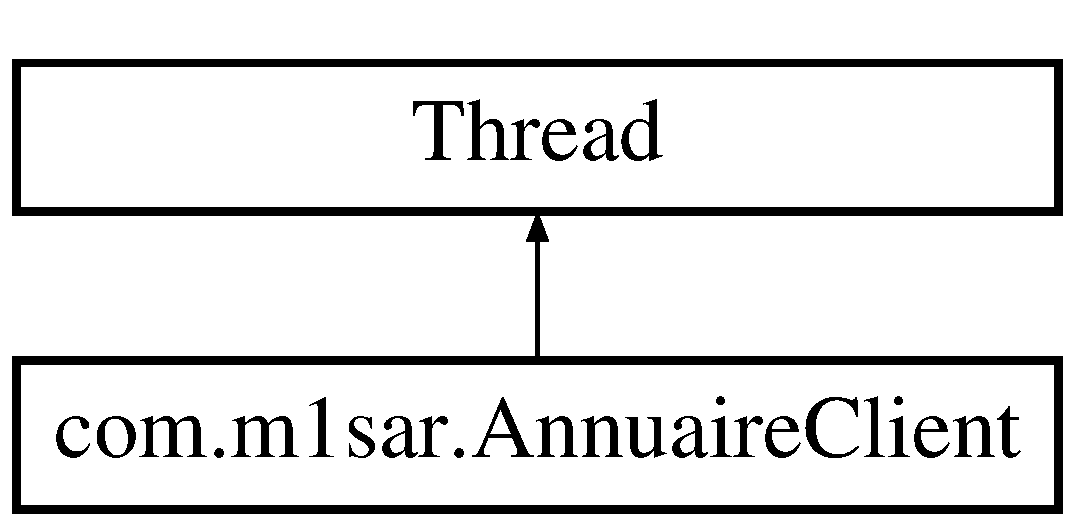
\includegraphics[height=2.000000cm]{classcom_1_1m1sar_1_1_annuaire_client}
\end{center}
\end{figure}
\subsection*{Public Member Functions}
\begin{DoxyCompactItemize}
\item 
\mbox{\Hypertarget{classcom_1_1m1sar_1_1_annuaire_client_a26d79864935f527b115ccecf5e966268}\label{classcom_1_1m1sar_1_1_annuaire_client_a26d79864935f527b115ccecf5e966268}} 
{\bfseries Annuaire\+Client} (int nport, Vector$<$ \hyperlink{classcom_1_1m1sar_1_1_thread_bourse}{Thread\+Bourse} $>$ courtiers)
\item 
\hyperlink{classcom_1_1m1sar_1_1_thread_bourse}{Thread\+Bourse} \hyperlink{classcom_1_1m1sar_1_1_annuaire_client_ac597ddd8b46c5fe7954f8d52039aa61b}{get\+Free\+Courtier} ()  throws Courtier\+Not\+Found\+Exception 
\item 
\mbox{\Hypertarget{classcom_1_1m1sar_1_1_annuaire_client_a9fb3d7b87893f2fa99b03b78dbcd964f}\label{classcom_1_1m1sar_1_1_annuaire_client_a9fb3d7b87893f2fa99b03b78dbcd964f}} 
void {\bfseries run} ()
\end{DoxyCompactItemize}


\subsection{Member Function Documentation}
\mbox{\Hypertarget{classcom_1_1m1sar_1_1_annuaire_client_ac597ddd8b46c5fe7954f8d52039aa61b}\label{classcom_1_1m1sar_1_1_annuaire_client_ac597ddd8b46c5fe7954f8d52039aa61b}} 
\index{com\+::m1sar\+::\+Annuaire\+Client@{com\+::m1sar\+::\+Annuaire\+Client}!get\+Free\+Courtier@{get\+Free\+Courtier}}
\index{get\+Free\+Courtier@{get\+Free\+Courtier}!com\+::m1sar\+::\+Annuaire\+Client@{com\+::m1sar\+::\+Annuaire\+Client}}
\subsubsection{\texorpdfstring{get\+Free\+Courtier()}{getFreeCourtier()}}
{\footnotesize\ttfamily \hyperlink{classcom_1_1m1sar_1_1_thread_bourse}{Thread\+Bourse} com.\+m1sar.\+Annuaire\+Client.\+get\+Free\+Courtier (\begin{DoxyParamCaption}{ }\end{DoxyParamCaption}) throws \hyperlink{classcom_1_1exceptions_1_1_courtier_not_found_exception}{Courtier\+Not\+Found\+Exception}}

\begin{DoxyAuthor}{Author}
Lyes Gets an avialable broker and sets it to the client 
\end{DoxyAuthor}

\begin{DoxyExceptions}{Exceptions}
{\em Courtier\+Not\+Found\+Exception} & \\
\hline
\end{DoxyExceptions}


The documentation for this class was generated from the following file\+:\begin{DoxyCompactItemize}
\item 
C\+:/\+Users/\+Nick/\+Desktop/\+M1 M\+I\+A\+G\+E/\+Iam\+The\+One/\+Systèmes \& Algo Répartis/\+Projet/sar/src/com/m1sar/Annuaire\+Client.\+java\end{DoxyCompactItemize}

\hypertarget{classcom_1_1m1sar_1_1_bourse}{}\section{com.\+m1sar.\+Bourse Class Reference}
\label{classcom_1_1m1sar_1_1_bourse}\index{com.\+m1sar.\+Bourse@{com.\+m1sar.\+Bourse}}
\subsection*{Public Member Functions}
\begin{DoxyCompactItemize}
\item 
Hash\+Map$<$ String, Double $>$ \hyperlink{classcom_1_1m1sar_1_1_bourse_a36588334a5398fdd07745a39ac809fa0}{update\+Price} ()
\item 
void \hyperlink{classcom_1_1m1sar_1_1_bourse_a04a69e51bbab147243a5b9f37fcc561a}{write\+To\+File} (Hash\+Map informations)
\item 
Hash\+Map$<$ String, Double $>$ \hyperlink{classcom_1_1m1sar_1_1_bourse_a807d02571a2cfdfccb83b74549a3e208}{read\+From\+File} (String filename)
\item 
\hyperlink{classcom_1_1m1sar_1_1_entreprise}{Entreprise} \hyperlink{classcom_1_1m1sar_1_1_bourse_a5b396735aca0672d7f37a2eb098f4edf}{get\+By\+Name} (String name)
\item 
\hyperlink{classcom_1_1m1sar_1_1_ordre}{Ordre} \hyperlink{classcom_1_1m1sar_1_1_bourse_aeb40be5d0f691a90eb1f6629f42e56de}{consommer} (String nom\+Courtier)
\item 
void \hyperlink{classcom_1_1m1sar_1_1_bourse_aa084f404d85f7292a1238ebc38ceac09}{accord} (String nom\+Courtier)  throws I\+O\+Exception 
\item 
boolean \hyperlink{classcom_1_1m1sar_1_1_bourse_a0bfccebb42e75ab2465b86ceb2ec9f68}{matching} (\hyperlink{classcom_1_1m1sar_1_1_ordre}{Ordre} achat, \hyperlink{classcom_1_1m1sar_1_1_ordre}{Ordre} vente)
\item 
void \hyperlink{classcom_1_1m1sar_1_1_bourse_a735c9da562fa5e84f2cc50cfed378bd9}{init\+Companies} ()
\item 
void \hyperlink{classcom_1_1m1sar_1_1_bourse_ae4e655b8d10208ff6b9e73eb62767558}{init\+Prix\+Par\+Entreprise} ()
\item 
Hash\+Map$<$ String, Double $>$ \hyperlink{classcom_1_1m1sar_1_1_bourse_ae68d9ea867f6e9043afe0b5868dda5fe}{get\+Prix\+Par\+Entreprise} ()
\item 
Vector$<$ \hyperlink{classcom_1_1m1sar_1_1_ordre}{Ordre} $>$ \hyperlink{classcom_1_1m1sar_1_1_bourse_acdeb99f593d0fdc0743934cb7e692156}{get\+Ordres} ()
\item 
void \hyperlink{classcom_1_1m1sar_1_1_bourse_a33e6699fa91c63f54221f1ebf3de723b}{set\+Ordres} (Vector$<$ \hyperlink{classcom_1_1m1sar_1_1_ordre}{Ordre} $>$ ordres)
\item 
\hyperlink{classcom_1_1m1sar_1_1_thread_bourse}{Thread\+Bourse} \hyperlink{classcom_1_1m1sar_1_1_bourse_a2c4daf19799b68d297a686df4aebb0c4}{get\+Thread\+By\+Name} (String nom\+TH)
\end{DoxyCompactItemize}
\subsection*{Static Public Member Functions}
\begin{DoxyCompactItemize}
\item 
\mbox{\Hypertarget{classcom_1_1m1sar_1_1_bourse_a5bbb0315c9e6fe1c74d6f112eefaf847}\label{classcom_1_1m1sar_1_1_bourse_a5bbb0315c9e6fe1c74d6f112eefaf847}} 
static void {\bfseries main} (String\mbox{[}$\,$\mbox{]} args)  throws I\+O\+Exception
\end{DoxyCompactItemize}


\subsection{Member Function Documentation}
\mbox{\Hypertarget{classcom_1_1m1sar_1_1_bourse_aa084f404d85f7292a1238ebc38ceac09}\label{classcom_1_1m1sar_1_1_bourse_aa084f404d85f7292a1238ebc38ceac09}} 
\index{com\+::m1sar\+::\+Bourse@{com\+::m1sar\+::\+Bourse}!accord@{accord}}
\index{accord@{accord}!com\+::m1sar\+::\+Bourse@{com\+::m1sar\+::\+Bourse}}
\subsubsection{\texorpdfstring{accord()}{accord()}}
{\footnotesize\ttfamily void com.\+m1sar.\+Bourse.\+accord (\begin{DoxyParamCaption}\item[{String}]{nom\+Courtier }\end{DoxyParamCaption}) throws I\+O\+Exception}

\begin{DoxyAuthor}{Author}
Lyes Gets and returns the order matching with the name of the Broker. 
\end{DoxyAuthor}

\begin{DoxyParams}{Parameters}
{\em nom\+Courtier} & \+: the name of broker \\
\hline
\end{DoxyParams}
\begin{DoxyReturn}{Returns}
{\ttfamily \hyperlink{classcom_1_1m1sar_1_1_ordre}{Ordre}} 
\end{DoxyReturn}
\mbox{\Hypertarget{classcom_1_1m1sar_1_1_bourse_aeb40be5d0f691a90eb1f6629f42e56de}\label{classcom_1_1m1sar_1_1_bourse_aeb40be5d0f691a90eb1f6629f42e56de}} 
\index{com\+::m1sar\+::\+Bourse@{com\+::m1sar\+::\+Bourse}!consommer@{consommer}}
\index{consommer@{consommer}!com\+::m1sar\+::\+Bourse@{com\+::m1sar\+::\+Bourse}}
\subsubsection{\texorpdfstring{consommer()}{consommer()}}
{\footnotesize\ttfamily \hyperlink{classcom_1_1m1sar_1_1_ordre}{Ordre} com.\+m1sar.\+Bourse.\+consommer (\begin{DoxyParamCaption}\item[{String}]{nom\+Courtier }\end{DoxyParamCaption})}

\begin{DoxyReturn}{Returns}
le premier ordre appertenant au client que traite le courtier nom\+Courtier 
\end{DoxyReturn}
\mbox{\Hypertarget{classcom_1_1m1sar_1_1_bourse_a5b396735aca0672d7f37a2eb098f4edf}\label{classcom_1_1m1sar_1_1_bourse_a5b396735aca0672d7f37a2eb098f4edf}} 
\index{com\+::m1sar\+::\+Bourse@{com\+::m1sar\+::\+Bourse}!get\+By\+Name@{get\+By\+Name}}
\index{get\+By\+Name@{get\+By\+Name}!com\+::m1sar\+::\+Bourse@{com\+::m1sar\+::\+Bourse}}
\subsubsection{\texorpdfstring{get\+By\+Name()}{getByName()}}
{\footnotesize\ttfamily \hyperlink{classcom_1_1m1sar_1_1_entreprise}{Entreprise} com.\+m1sar.\+Bourse.\+get\+By\+Name (\begin{DoxyParamCaption}\item[{String}]{name }\end{DoxyParamCaption})}

\begin{DoxyAuthor}{Author}
Lyes Gets and returns the Company matching with the name passed as argument. 
\end{DoxyAuthor}

\begin{DoxyParams}{Parameters}
{\em name} & \+: the name of the company \\
\hline
\end{DoxyParams}
\begin{DoxyReturn}{Returns}
{\ttfamily \hyperlink{classcom_1_1m1sar_1_1_entreprise}{Entreprise}} 
\end{DoxyReturn}

\begin{DoxyExceptions}{Exceptions}
{\em No\+Such\+Element\+Exception} & if the name does not match with all companies \\
\hline
\end{DoxyExceptions}
\mbox{\Hypertarget{classcom_1_1m1sar_1_1_bourse_acdeb99f593d0fdc0743934cb7e692156}\label{classcom_1_1m1sar_1_1_bourse_acdeb99f593d0fdc0743934cb7e692156}} 
\index{com\+::m1sar\+::\+Bourse@{com\+::m1sar\+::\+Bourse}!get\+Ordres@{get\+Ordres}}
\index{get\+Ordres@{get\+Ordres}!com\+::m1sar\+::\+Bourse@{com\+::m1sar\+::\+Bourse}}
\subsubsection{\texorpdfstring{get\+Ordres()}{getOrdres()}}
{\footnotesize\ttfamily Vector$<$\hyperlink{classcom_1_1m1sar_1_1_ordre}{Ordre}$>$ com.\+m1sar.\+Bourse.\+get\+Ordres (\begin{DoxyParamCaption}{ }\end{DoxyParamCaption})}

\begin{DoxyAuthor}{Author}
Lyes Returns the vector of Orders 
\end{DoxyAuthor}
\begin{DoxyReturn}{Returns}
{\ttfamily void} 
\end{DoxyReturn}
\mbox{\Hypertarget{classcom_1_1m1sar_1_1_bourse_ae68d9ea867f6e9043afe0b5868dda5fe}\label{classcom_1_1m1sar_1_1_bourse_ae68d9ea867f6e9043afe0b5868dda5fe}} 
\index{com\+::m1sar\+::\+Bourse@{com\+::m1sar\+::\+Bourse}!get\+Prix\+Par\+Entreprise@{get\+Prix\+Par\+Entreprise}}
\index{get\+Prix\+Par\+Entreprise@{get\+Prix\+Par\+Entreprise}!com\+::m1sar\+::\+Bourse@{com\+::m1sar\+::\+Bourse}}
\subsubsection{\texorpdfstring{get\+Prix\+Par\+Entreprise()}{getPrixParEntreprise()}}
{\footnotesize\ttfamily Hash\+Map$<$String, Double$>$ com.\+m1sar.\+Bourse.\+get\+Prix\+Par\+Entreprise (\begin{DoxyParamCaption}{ }\end{DoxyParamCaption})}

\begin{DoxyAuthor}{Author}
Lyes Returns the hash\+Map that shows the price of an action for each company 
\end{DoxyAuthor}
\begin{DoxyReturn}{Returns}
{\ttfamily void} 
\end{DoxyReturn}
\mbox{\Hypertarget{classcom_1_1m1sar_1_1_bourse_a2c4daf19799b68d297a686df4aebb0c4}\label{classcom_1_1m1sar_1_1_bourse_a2c4daf19799b68d297a686df4aebb0c4}} 
\index{com\+::m1sar\+::\+Bourse@{com\+::m1sar\+::\+Bourse}!get\+Thread\+By\+Name@{get\+Thread\+By\+Name}}
\index{get\+Thread\+By\+Name@{get\+Thread\+By\+Name}!com\+::m1sar\+::\+Bourse@{com\+::m1sar\+::\+Bourse}}
\subsubsection{\texorpdfstring{get\+Thread\+By\+Name()}{getThreadByName()}}
{\footnotesize\ttfamily \hyperlink{classcom_1_1m1sar_1_1_thread_bourse}{Thread\+Bourse} com.\+m1sar.\+Bourse.\+get\+Thread\+By\+Name (\begin{DoxyParamCaption}\item[{String}]{nom\+TH }\end{DoxyParamCaption})}

\begin{DoxyAuthor}{Author}
Lyes Returns the Broker from its name 
\end{DoxyAuthor}

\begin{DoxyParams}{Parameters}
{\em the} & Name (id) of the Broker to be returned \\
\hline
\end{DoxyParams}
\begin{DoxyReturn}{Returns}
{\ttfamily \hyperlink{classcom_1_1m1sar_1_1_thread_bourse}{Thread\+Bourse}} 
\end{DoxyReturn}
\mbox{\Hypertarget{classcom_1_1m1sar_1_1_bourse_a735c9da562fa5e84f2cc50cfed378bd9}\label{classcom_1_1m1sar_1_1_bourse_a735c9da562fa5e84f2cc50cfed378bd9}} 
\index{com\+::m1sar\+::\+Bourse@{com\+::m1sar\+::\+Bourse}!init\+Companies@{init\+Companies}}
\index{init\+Companies@{init\+Companies}!com\+::m1sar\+::\+Bourse@{com\+::m1sar\+::\+Bourse}}
\subsubsection{\texorpdfstring{init\+Companies()}{initCompanies()}}
{\footnotesize\ttfamily void com.\+m1sar.\+Bourse.\+init\+Companies (\begin{DoxyParamCaption}{ }\end{DoxyParamCaption})}

\begin{DoxyAuthor}{Author}
Lyes Initializes with a list of companies, and the prices for each company 
\end{DoxyAuthor}
\begin{DoxyReturn}{Returns}
{\ttfamily void} 
\end{DoxyReturn}
\mbox{\Hypertarget{classcom_1_1m1sar_1_1_bourse_ae4e655b8d10208ff6b9e73eb62767558}\label{classcom_1_1m1sar_1_1_bourse_ae4e655b8d10208ff6b9e73eb62767558}} 
\index{com\+::m1sar\+::\+Bourse@{com\+::m1sar\+::\+Bourse}!init\+Prix\+Par\+Entreprise@{init\+Prix\+Par\+Entreprise}}
\index{init\+Prix\+Par\+Entreprise@{init\+Prix\+Par\+Entreprise}!com\+::m1sar\+::\+Bourse@{com\+::m1sar\+::\+Bourse}}
\subsubsection{\texorpdfstring{init\+Prix\+Par\+Entreprise()}{initPrixParEntreprise()}}
{\footnotesize\ttfamily void com.\+m1sar.\+Bourse.\+init\+Prix\+Par\+Entreprise (\begin{DoxyParamCaption}{ }\end{DoxyParamCaption})}

\begin{DoxyAuthor}{Author}
Lyes Initializes the prices for each company 
\end{DoxyAuthor}
\begin{DoxyReturn}{Returns}
{\ttfamily void} 
\end{DoxyReturn}
\mbox{\Hypertarget{classcom_1_1m1sar_1_1_bourse_a0bfccebb42e75ab2465b86ceb2ec9f68}\label{classcom_1_1m1sar_1_1_bourse_a0bfccebb42e75ab2465b86ceb2ec9f68}} 
\index{com\+::m1sar\+::\+Bourse@{com\+::m1sar\+::\+Bourse}!matching@{matching}}
\index{matching@{matching}!com\+::m1sar\+::\+Bourse@{com\+::m1sar\+::\+Bourse}}
\subsubsection{\texorpdfstring{matching()}{matching()}}
{\footnotesize\ttfamily boolean com.\+m1sar.\+Bourse.\+matching (\begin{DoxyParamCaption}\item[{\hyperlink{classcom_1_1m1sar_1_1_ordre}{Ordre}}]{achat,  }\item[{\hyperlink{classcom_1_1m1sar_1_1_ordre}{Ordre}}]{vente }\end{DoxyParamCaption})}

\begin{DoxyAuthor}{Author}
Lyes Checks if the buying order matchs with the selling order, returns true if so. 
\end{DoxyAuthor}

\begin{DoxyParams}{Parameters}
{\em achat} & \+: the buying order \\
\hline
{\em vente} & \+: the selling order \\
\hline
\end{DoxyParams}
\begin{DoxyReturn}{Returns}
{\ttfamily boolean} 
\end{DoxyReturn}
\mbox{\Hypertarget{classcom_1_1m1sar_1_1_bourse_a807d02571a2cfdfccb83b74549a3e208}\label{classcom_1_1m1sar_1_1_bourse_a807d02571a2cfdfccb83b74549a3e208}} 
\index{com\+::m1sar\+::\+Bourse@{com\+::m1sar\+::\+Bourse}!read\+From\+File@{read\+From\+File}}
\index{read\+From\+File@{read\+From\+File}!com\+::m1sar\+::\+Bourse@{com\+::m1sar\+::\+Bourse}}
\subsubsection{\texorpdfstring{read\+From\+File()}{readFromFile()}}
{\footnotesize\ttfamily Hash\+Map$<$String,Double$>$ com.\+m1sar.\+Bourse.\+read\+From\+File (\begin{DoxyParamCaption}\item[{String}]{filename }\end{DoxyParamCaption})}

\begin{DoxyAuthor}{Author}
Lyes Reads from file the history 
\end{DoxyAuthor}
\mbox{\Hypertarget{classcom_1_1m1sar_1_1_bourse_a33e6699fa91c63f54221f1ebf3de723b}\label{classcom_1_1m1sar_1_1_bourse_a33e6699fa91c63f54221f1ebf3de723b}} 
\index{com\+::m1sar\+::\+Bourse@{com\+::m1sar\+::\+Bourse}!set\+Ordres@{set\+Ordres}}
\index{set\+Ordres@{set\+Ordres}!com\+::m1sar\+::\+Bourse@{com\+::m1sar\+::\+Bourse}}
\subsubsection{\texorpdfstring{set\+Ordres()}{setOrdres()}}
{\footnotesize\ttfamily void com.\+m1sar.\+Bourse.\+set\+Ordres (\begin{DoxyParamCaption}\item[{Vector$<$ \hyperlink{classcom_1_1m1sar_1_1_ordre}{Ordre} $>$}]{ordres }\end{DoxyParamCaption})}

\begin{DoxyAuthor}{Author}
Lyes Sets the orders for the market 
\end{DoxyAuthor}

\begin{DoxyParams}{Parameters}
{\em the} & vector of orders to be set \\
\hline
\end{DoxyParams}
\begin{DoxyReturn}{Returns}
{\ttfamily void} 
\end{DoxyReturn}
\mbox{\Hypertarget{classcom_1_1m1sar_1_1_bourse_a36588334a5398fdd07745a39ac809fa0}\label{classcom_1_1m1sar_1_1_bourse_a36588334a5398fdd07745a39ac809fa0}} 
\index{com\+::m1sar\+::\+Bourse@{com\+::m1sar\+::\+Bourse}!update\+Price@{update\+Price}}
\index{update\+Price@{update\+Price}!com\+::m1sar\+::\+Bourse@{com\+::m1sar\+::\+Bourse}}
\subsubsection{\texorpdfstring{update\+Price()}{updatePrice()}}
{\footnotesize\ttfamily Hash\+Map$<$String,Double$>$ com.\+m1sar.\+Bourse.\+update\+Price (\begin{DoxyParamCaption}{ }\end{DoxyParamCaption})}

\begin{DoxyAuthor}{Author}
Lyes At the end of the day, update the price of every business action in each company Follow this rule \+: new price = old prince + delta where delta = (number of purchase orders -\/ number of sale orders ) / number of buisness actions 
\end{DoxyAuthor}
\mbox{\Hypertarget{classcom_1_1m1sar_1_1_bourse_a04a69e51bbab147243a5b9f37fcc561a}\label{classcom_1_1m1sar_1_1_bourse_a04a69e51bbab147243a5b9f37fcc561a}} 
\index{com\+::m1sar\+::\+Bourse@{com\+::m1sar\+::\+Bourse}!write\+To\+File@{write\+To\+File}}
\index{write\+To\+File@{write\+To\+File}!com\+::m1sar\+::\+Bourse@{com\+::m1sar\+::\+Bourse}}
\subsubsection{\texorpdfstring{write\+To\+File()}{writeToFile()}}
{\footnotesize\ttfamily void com.\+m1sar.\+Bourse.\+write\+To\+File (\begin{DoxyParamCaption}\item[{Hash\+Map}]{informations }\end{DoxyParamCaption})}

\begin{DoxyAuthor}{Author}
Lyes At the end of the day, saves the informations serialized to a file 
\end{DoxyAuthor}


The documentation for this class was generated from the following file\+:\begin{DoxyCompactItemize}
\item 
C\+:/\+Users/\+Nick/\+Desktop/\+M1 M\+I\+A\+G\+E/\+Iam\+The\+One/\+Systèmes \& Algo Répartis/\+Projet/sar/src/com/m1sar/Bourse.\+java\end{DoxyCompactItemize}

\hypertarget{classcom_1_1m1sar_1_1_client}{}\section{com.\+m1sar.\+Client Class Reference}
\label{classcom_1_1m1sar_1_1_client}\index{com.\+m1sar.\+Client@{com.\+m1sar.\+Client}}
\subsection*{Public Member Functions}
\begin{DoxyCompactItemize}
\item 
\mbox{\Hypertarget{classcom_1_1m1sar_1_1_client_af679443c7353bb7bbd197cf94049a70c}\label{classcom_1_1m1sar_1_1_client_af679443c7353bb7bbd197cf94049a70c}} 
{\bfseries Client} (String name\+Client, double solde, int port, Inet\+Address hte)
\item 
void \hyperlink{classcom_1_1m1sar_1_1_client_aeff9ee8926647a8be490c5f0beea31d5}{connexion} ()
\item 
void \hyperlink{classcom_1_1m1sar_1_1_client_ac6681e529e1a045aae86e571dbfea5e3}{inscription} ()
\item 
\hyperlink{classcom_1_1m1sar_1_1_ordre}{Ordre} \hyperlink{classcom_1_1m1sar_1_1_client_a7042e50f398b3b9b7bbeada8f12954c2}{acheter} (double prix, int quantite, String entreprise)
\item 
\hyperlink{classcom_1_1m1sar_1_1_ordre}{Ordre} \hyperlink{classcom_1_1m1sar_1_1_client_ac7c456af1862320de2c394a23a7d80cd}{vendre} (double prix, int quantite, String entreprise)
\item 
void \hyperlink{classcom_1_1m1sar_1_1_client_a661a6a21b9891b99319d45fe1bb7c0c9}{echange\+Ordres\+Client\+Courtier} ()
\item 
boolean \hyperlink{classcom_1_1m1sar_1_1_client_a193f812c6df9bd999c444eb3ec5007da}{vente\+Legal} (String entreprise, int quantite)
\item 
boolean \hyperlink{classcom_1_1m1sar_1_1_client_a9ab9d2ee49a49ffc34d876c554bf29b3}{achat\+Legal} (String entreprise, double prix, int quantite)
\item 
void \hyperlink{classcom_1_1m1sar_1_1_client_adbad3a491bebe1acf093c0c6343ec507}{deconnexion} ()
\item 
\hyperlink{classcom_1_1m1sar_1_1_ordre}{Ordre} \hyperlink{classcom_1_1m1sar_1_1_client_a29230c6248c0b37d1faeb254270f0001}{get\+Order\+By\+Id} (int id)
\item 
void \hyperlink{classcom_1_1m1sar_1_1_client_a78ef39501ca822bcd7df390bead5baae}{get\+Reponse\+Bource} (int id\+Ordre, boolean yes\+Ou\+Non)
\item 
void \hyperlink{classcom_1_1m1sar_1_1_client_ae58f81c93ca69cc75c923e91f758d75f}{maj\+Portefeuille\+Achat} (\hyperlink{classcom_1_1m1sar_1_1_ordre}{Ordre} r)
\item 
void \hyperlink{classcom_1_1m1sar_1_1_client_afa011fd42124137bc9131ae8b9f2851d}{maj\+Portefeuille\+Vente} (\hyperlink{classcom_1_1m1sar_1_1_ordre}{Ordre} r)
\item 
void \hyperlink{classcom_1_1m1sar_1_1_client_a289d7402a20981f2ab07159e617ec3d8}{read\+State\+Stocks} ()
\item 
void \hyperlink{classcom_1_1m1sar_1_1_client_af8ee1c17e73359f447bc14b8fe4b790c}{Produir} (\hyperlink{classcom_1_1m1sar_1_1_ordre}{Ordre} r)
\end{DoxyCompactItemize}
\subsection*{Static Public Member Functions}
\begin{DoxyCompactItemize}
\item 
\mbox{\Hypertarget{classcom_1_1m1sar_1_1_client_a952cf270821d658eef12c5dca9d16133}\label{classcom_1_1m1sar_1_1_client_a952cf270821d658eef12c5dca9d16133}} 
static void {\bfseries main} (String\mbox{[}$\,$\mbox{]} args)  throws Unknown\+Host\+Exception
\end{DoxyCompactItemize}
\subsection*{Static Public Attributes}
\begin{DoxyCompactItemize}
\item 
\mbox{\Hypertarget{classcom_1_1m1sar_1_1_client_afea2b8c72db2abdc5d6e68e5d817bc25}\label{classcom_1_1m1sar_1_1_client_afea2b8c72db2abdc5d6e68e5d817bc25}} 
static int {\bfseries cpt} =0
\end{DoxyCompactItemize}


\subsection{Detailed Description}
\begin{DoxyAuthor}{Author}
Vitalina La classe \hyperlink{classcom_1_1m1sar_1_1_client}{Client} qui peut acheter ou vendre des actions 
\end{DoxyAuthor}


\subsection{Member Function Documentation}
\mbox{\Hypertarget{classcom_1_1m1sar_1_1_client_a9ab9d2ee49a49ffc34d876c554bf29b3}\label{classcom_1_1m1sar_1_1_client_a9ab9d2ee49a49ffc34d876c554bf29b3}} 
\index{com\+::m1sar\+::\+Client@{com\+::m1sar\+::\+Client}!achat\+Legal@{achat\+Legal}}
\index{achat\+Legal@{achat\+Legal}!com\+::m1sar\+::\+Client@{com\+::m1sar\+::\+Client}}
\subsubsection{\texorpdfstring{achat\+Legal()}{achatLegal()}}
{\footnotesize\ttfamily boolean com.\+m1sar.\+Client.\+achat\+Legal (\begin{DoxyParamCaption}\item[{String}]{entreprise,  }\item[{double}]{prix,  }\item[{int}]{quantite }\end{DoxyParamCaption})}

\begin{DoxyAuthor}{Author}
Vitalina 
\end{DoxyAuthor}

\begin{DoxyParams}{Parameters}
{\em name} & of company and the price of all Stocks which \hyperlink{classcom_1_1m1sar_1_1_client}{Client} want to buy \\
\hline
\end{DoxyParams}
\begin{DoxyReturn}{Returns}
true or false check if the condition is legal to buy \hyperlink{classcom_1_1m1sar_1_1_ordre_achat}{Ordre\+Achat} 
\end{DoxyReturn}
\mbox{\Hypertarget{classcom_1_1m1sar_1_1_client_a7042e50f398b3b9b7bbeada8f12954c2}\label{classcom_1_1m1sar_1_1_client_a7042e50f398b3b9b7bbeada8f12954c2}} 
\index{com\+::m1sar\+::\+Client@{com\+::m1sar\+::\+Client}!acheter@{acheter}}
\index{acheter@{acheter}!com\+::m1sar\+::\+Client@{com\+::m1sar\+::\+Client}}
\subsubsection{\texorpdfstring{acheter()}{acheter()}}
{\footnotesize\ttfamily \hyperlink{classcom_1_1m1sar_1_1_ordre}{Ordre} com.\+m1sar.\+Client.\+acheter (\begin{DoxyParamCaption}\item[{double}]{prix,  }\item[{int}]{quantite,  }\item[{String}]{entreprise }\end{DoxyParamCaption})}

\begin{DoxyAuthor}{Author}
Vitalina 
\end{DoxyAuthor}

\begin{DoxyParams}{Parameters}
{\em clients} & price ,amount how much he wants to buy of stocks, name of company \\
\hline
\end{DoxyParams}
\begin{DoxyReturn}{Returns}
\hyperlink{classcom_1_1m1sar_1_1_ordre_achat}{Ordre\+Achat} if it is legal or non return null 
\end{DoxyReturn}
\mbox{\Hypertarget{classcom_1_1m1sar_1_1_client_aeff9ee8926647a8be490c5f0beea31d5}\label{classcom_1_1m1sar_1_1_client_aeff9ee8926647a8be490c5f0beea31d5}} 
\index{com\+::m1sar\+::\+Client@{com\+::m1sar\+::\+Client}!connexion@{connexion}}
\index{connexion@{connexion}!com\+::m1sar\+::\+Client@{com\+::m1sar\+::\+Client}}
\subsubsection{\texorpdfstring{connexion()}{connexion()}}
{\footnotesize\ttfamily void com.\+m1sar.\+Client.\+connexion (\begin{DoxyParamCaption}{ }\end{DoxyParamCaption})}

\begin{DoxyAuthor}{Author}
Vitalina make connection with Thread\+Bource which find for this client \hyperlink{classcom_1_1m1sar_1_1_courtier}{Courtier} available and client obtain IP and host of this \hyperlink{classcom_1_1m1sar_1_1_courtier}{Courtier} if any \hyperlink{classcom_1_1m1sar_1_1_courtier}{Courtier} is available client is disconnected 
\end{DoxyAuthor}
\mbox{\Hypertarget{classcom_1_1m1sar_1_1_client_adbad3a491bebe1acf093c0c6343ec507}\label{classcom_1_1m1sar_1_1_client_adbad3a491bebe1acf093c0c6343ec507}} 
\index{com\+::m1sar\+::\+Client@{com\+::m1sar\+::\+Client}!deconnexion@{deconnexion}}
\index{deconnexion@{deconnexion}!com\+::m1sar\+::\+Client@{com\+::m1sar\+::\+Client}}
\subsubsection{\texorpdfstring{deconnexion()}{deconnexion()}}
{\footnotesize\ttfamily void com.\+m1sar.\+Client.\+deconnexion (\begin{DoxyParamCaption}{ }\end{DoxyParamCaption})}

\begin{DoxyAuthor}{Author}
Vitalina disconnection of \hyperlink{classcom_1_1m1sar_1_1_client}{Client} 
\end{DoxyAuthor}
\mbox{\Hypertarget{classcom_1_1m1sar_1_1_client_a661a6a21b9891b99319d45fe1bb7c0c9}\label{classcom_1_1m1sar_1_1_client_a661a6a21b9891b99319d45fe1bb7c0c9}} 
\index{com\+::m1sar\+::\+Client@{com\+::m1sar\+::\+Client}!echange\+Ordres\+Client\+Courtier@{echange\+Ordres\+Client\+Courtier}}
\index{echange\+Ordres\+Client\+Courtier@{echange\+Ordres\+Client\+Courtier}!com\+::m1sar\+::\+Client@{com\+::m1sar\+::\+Client}}
\subsubsection{\texorpdfstring{echange\+Ordres\+Client\+Courtier()}{echangeOrdresClientCourtier()}}
{\footnotesize\ttfamily void com.\+m1sar.\+Client.\+echange\+Ordres\+Client\+Courtier (\begin{DoxyParamCaption}{ }\end{DoxyParamCaption})}

\begin{DoxyAuthor}{Author}
Vitalina make exchanges between \hyperlink{classcom_1_1m1sar_1_1_client}{Client}, \hyperlink{classcom_1_1m1sar_1_1_courtier}{Courtier} and \hyperlink{classcom_1_1m1sar_1_1_thread_bourse}{Thread\+Bourse} and received notifications if Orders were accepted or non and finally disconnection of this client 
\end{DoxyAuthor}
\mbox{\Hypertarget{classcom_1_1m1sar_1_1_client_a29230c6248c0b37d1faeb254270f0001}\label{classcom_1_1m1sar_1_1_client_a29230c6248c0b37d1faeb254270f0001}} 
\index{com\+::m1sar\+::\+Client@{com\+::m1sar\+::\+Client}!get\+Order\+By\+Id@{get\+Order\+By\+Id}}
\index{get\+Order\+By\+Id@{get\+Order\+By\+Id}!com\+::m1sar\+::\+Client@{com\+::m1sar\+::\+Client}}
\subsubsection{\texorpdfstring{get\+Order\+By\+Id()}{getOrderById()}}
{\footnotesize\ttfamily \hyperlink{classcom_1_1m1sar_1_1_ordre}{Ordre} com.\+m1sar.\+Client.\+get\+Order\+By\+Id (\begin{DoxyParamCaption}\item[{int}]{id }\end{DoxyParamCaption})}

\begin{DoxyAuthor}{Author}
Vitalina 
\end{DoxyAuthor}

\begin{DoxyParams}{Parameters}
{\em id} & of Order \\
\hline
\end{DoxyParams}
\begin{DoxyReturn}{Returns}
Order from list of orders 
\end{DoxyReturn}
\mbox{\Hypertarget{classcom_1_1m1sar_1_1_client_a78ef39501ca822bcd7df390bead5baae}\label{classcom_1_1m1sar_1_1_client_a78ef39501ca822bcd7df390bead5baae}} 
\index{com\+::m1sar\+::\+Client@{com\+::m1sar\+::\+Client}!get\+Reponse\+Bource@{get\+Reponse\+Bource}}
\index{get\+Reponse\+Bource@{get\+Reponse\+Bource}!com\+::m1sar\+::\+Client@{com\+::m1sar\+::\+Client}}
\subsubsection{\texorpdfstring{get\+Reponse\+Bource()}{getReponseBource()}}
{\footnotesize\ttfamily void com.\+m1sar.\+Client.\+get\+Reponse\+Bource (\begin{DoxyParamCaption}\item[{int}]{id\+Ordre,  }\item[{boolean}]{yes\+Ou\+Non }\end{DoxyParamCaption})}

\begin{DoxyAuthor}{Author}
Vitalina 
\end{DoxyAuthor}

\begin{DoxyParams}{Parameters}
{\em id} & of Order, boolean if Order was accepted or no deals answer of \hyperlink{classcom_1_1m1sar_1_1_bourse}{Bourse} and update portefeille according to Order\+Vante or Order\+Achat \\
\hline
\end{DoxyParams}
\mbox{\Hypertarget{classcom_1_1m1sar_1_1_client_ac6681e529e1a045aae86e571dbfea5e3}\label{classcom_1_1m1sar_1_1_client_ac6681e529e1a045aae86e571dbfea5e3}} 
\index{com\+::m1sar\+::\+Client@{com\+::m1sar\+::\+Client}!inscription@{inscription}}
\index{inscription@{inscription}!com\+::m1sar\+::\+Client@{com\+::m1sar\+::\+Client}}
\subsubsection{\texorpdfstring{inscription()}{inscription()}}
{\footnotesize\ttfamily void com.\+m1sar.\+Client.\+inscription (\begin{DoxyParamCaption}{ }\end{DoxyParamCaption})}

\begin{DoxyAuthor}{Author}
Vitalina sends the Clients name to the \hyperlink{classcom_1_1m1sar_1_1_courtier}{Courtier} 
\end{DoxyAuthor}
\mbox{\Hypertarget{classcom_1_1m1sar_1_1_client_ae58f81c93ca69cc75c923e91f758d75f}\label{classcom_1_1m1sar_1_1_client_ae58f81c93ca69cc75c923e91f758d75f}} 
\index{com\+::m1sar\+::\+Client@{com\+::m1sar\+::\+Client}!maj\+Portefeuille\+Achat@{maj\+Portefeuille\+Achat}}
\index{maj\+Portefeuille\+Achat@{maj\+Portefeuille\+Achat}!com\+::m1sar\+::\+Client@{com\+::m1sar\+::\+Client}}
\subsubsection{\texorpdfstring{maj\+Portefeuille\+Achat()}{majPortefeuilleAchat()}}
{\footnotesize\ttfamily void com.\+m1sar.\+Client.\+maj\+Portefeuille\+Achat (\begin{DoxyParamCaption}\item[{\hyperlink{classcom_1_1m1sar_1_1_ordre}{Ordre}}]{r }\end{DoxyParamCaption})}

\begin{DoxyAuthor}{Author}
Vitalina Once the order is finished, updates the wallet of the current client only 
\end{DoxyAuthor}

\begin{DoxyParams}{Parameters}
{\em \hyperlink{classcom_1_1m1sar_1_1_ordre}{Ordre}} & \+: Buying order \\
\hline
\end{DoxyParams}
\mbox{\Hypertarget{classcom_1_1m1sar_1_1_client_afa011fd42124137bc9131ae8b9f2851d}\label{classcom_1_1m1sar_1_1_client_afa011fd42124137bc9131ae8b9f2851d}} 
\index{com\+::m1sar\+::\+Client@{com\+::m1sar\+::\+Client}!maj\+Portefeuille\+Vente@{maj\+Portefeuille\+Vente}}
\index{maj\+Portefeuille\+Vente@{maj\+Portefeuille\+Vente}!com\+::m1sar\+::\+Client@{com\+::m1sar\+::\+Client}}
\subsubsection{\texorpdfstring{maj\+Portefeuille\+Vente()}{majPortefeuilleVente()}}
{\footnotesize\ttfamily void com.\+m1sar.\+Client.\+maj\+Portefeuille\+Vente (\begin{DoxyParamCaption}\item[{\hyperlink{classcom_1_1m1sar_1_1_ordre}{Ordre}}]{r }\end{DoxyParamCaption})}

\begin{DoxyAuthor}{Author}
Vitalina Once the order is finished, updates the wallet of the current client only 
\end{DoxyAuthor}

\begin{DoxyParams}{Parameters}
{\em \hyperlink{classcom_1_1m1sar_1_1_ordre}{Ordre}} & \+: Selling order \\
\hline
\end{DoxyParams}
\mbox{\Hypertarget{classcom_1_1m1sar_1_1_client_af8ee1c17e73359f447bc14b8fe4b790c}\label{classcom_1_1m1sar_1_1_client_af8ee1c17e73359f447bc14b8fe4b790c}} 
\index{com\+::m1sar\+::\+Client@{com\+::m1sar\+::\+Client}!Produir@{Produir}}
\index{Produir@{Produir}!com\+::m1sar\+::\+Client@{com\+::m1sar\+::\+Client}}
\subsubsection{\texorpdfstring{Produir()}{Produir()}}
{\footnotesize\ttfamily void com.\+m1sar.\+Client.\+Produir (\begin{DoxyParamCaption}\item[{\hyperlink{classcom_1_1m1sar_1_1_ordre}{Ordre}}]{r }\end{DoxyParamCaption})}

\begin{DoxyAuthor}{Author}
Vitalina Sends an order to the Broker 
\end{DoxyAuthor}

\begin{DoxyParams}{Parameters}
{\em \hyperlink{classcom_1_1m1sar_1_1_ordre}{Ordre}} & \\
\hline
\end{DoxyParams}
\mbox{\Hypertarget{classcom_1_1m1sar_1_1_client_a289d7402a20981f2ab07159e617ec3d8}\label{classcom_1_1m1sar_1_1_client_a289d7402a20981f2ab07159e617ec3d8}} 
\index{com\+::m1sar\+::\+Client@{com\+::m1sar\+::\+Client}!read\+State\+Stocks@{read\+State\+Stocks}}
\index{read\+State\+Stocks@{read\+State\+Stocks}!com\+::m1sar\+::\+Client@{com\+::m1sar\+::\+Client}}
\subsubsection{\texorpdfstring{read\+State\+Stocks()}{readStateStocks()}}
{\footnotesize\ttfamily void com.\+m1sar.\+Client.\+read\+State\+Stocks (\begin{DoxyParamCaption}{ }\end{DoxyParamCaption})}

\begin{DoxyAuthor}{Author}
Vitalina Shows the market status to the client 
\end{DoxyAuthor}
\mbox{\Hypertarget{classcom_1_1m1sar_1_1_client_ac7c456af1862320de2c394a23a7d80cd}\label{classcom_1_1m1sar_1_1_client_ac7c456af1862320de2c394a23a7d80cd}} 
\index{com\+::m1sar\+::\+Client@{com\+::m1sar\+::\+Client}!vendre@{vendre}}
\index{vendre@{vendre}!com\+::m1sar\+::\+Client@{com\+::m1sar\+::\+Client}}
\subsubsection{\texorpdfstring{vendre()}{vendre()}}
{\footnotesize\ttfamily \hyperlink{classcom_1_1m1sar_1_1_ordre}{Ordre} com.\+m1sar.\+Client.\+vendre (\begin{DoxyParamCaption}\item[{double}]{prix,  }\item[{int}]{quantite,  }\item[{String}]{entreprise }\end{DoxyParamCaption})}

\begin{DoxyAuthor}{Author}
Vitalina 
\end{DoxyAuthor}

\begin{DoxyParams}{Parameters}
{\em clients} & price ,amount how much he wants to sale of stocks, name of company \\
\hline
\end{DoxyParams}
\begin{DoxyReturn}{Returns}
\hyperlink{classcom_1_1m1sar_1_1_ordre_vente}{Ordre\+Vente} if it is legal or non return null 
\end{DoxyReturn}
\mbox{\Hypertarget{classcom_1_1m1sar_1_1_client_a193f812c6df9bd999c444eb3ec5007da}\label{classcom_1_1m1sar_1_1_client_a193f812c6df9bd999c444eb3ec5007da}} 
\index{com\+::m1sar\+::\+Client@{com\+::m1sar\+::\+Client}!vente\+Legal@{vente\+Legal}}
\index{vente\+Legal@{vente\+Legal}!com\+::m1sar\+::\+Client@{com\+::m1sar\+::\+Client}}
\subsubsection{\texorpdfstring{vente\+Legal()}{venteLegal()}}
{\footnotesize\ttfamily boolean com.\+m1sar.\+Client.\+vente\+Legal (\begin{DoxyParamCaption}\item[{String}]{entreprise,  }\item[{int}]{quantite }\end{DoxyParamCaption})}

\begin{DoxyAuthor}{Author}
Vitalina 
\end{DoxyAuthor}

\begin{DoxyParams}{Parameters}
{\em name} & of company and the number of Stocks to buy \\
\hline
\end{DoxyParams}
\begin{DoxyReturn}{Returns}
true or false check if the condition is legal to sell \hyperlink{classcom_1_1m1sar_1_1_ordre_vente}{Ordre\+Vente} 
\end{DoxyReturn}


The documentation for this class was generated from the following file\+:\begin{DoxyCompactItemize}
\item 
C\+:/\+Users/\+Nick/\+Desktop/\+M1 M\+I\+A\+G\+E/\+Iam\+The\+One/\+Systèmes \& Algo Répartis/\+Projet/sar/src/com/m1sar/Client.\+java\end{DoxyCompactItemize}

\hypertarget{classcom_1_1m1sar_1_1_courtier}{}\section{com.\+m1sar.\+Courtier Class Reference}
\label{classcom_1_1m1sar_1_1_courtier}\index{com.\+m1sar.\+Courtier@{com.\+m1sar.\+Courtier}}
Inheritance diagram for com.\+m1sar.\+Courtier\+:\begin{figure}[H]
\begin{center}
\leavevmode
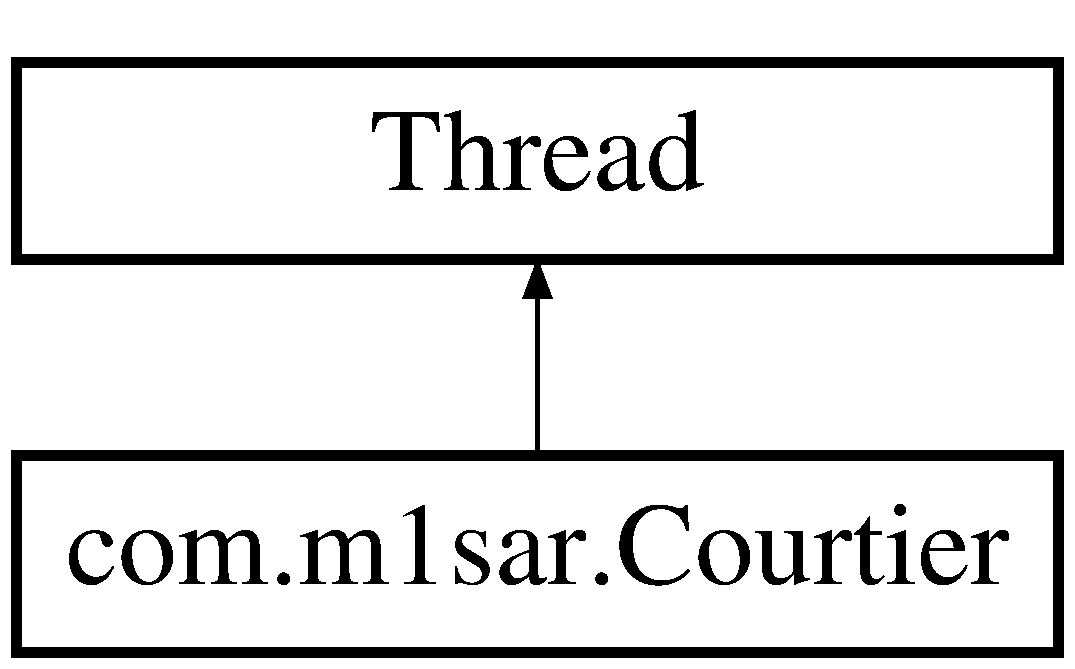
\includegraphics[height=2.000000cm]{classcom_1_1m1sar_1_1_courtier}
\end{center}
\end{figure}
\subsection*{Public Member Functions}
\begin{DoxyCompactItemize}
\item 
\mbox{\Hypertarget{classcom_1_1m1sar_1_1_courtier_aace4acdb7a996a617f18e7073472db99}\label{classcom_1_1m1sar_1_1_courtier_aace4acdb7a996a617f18e7073472db99}} 
{\bfseries Courtier} (String name, int port, Inet\+Address hte)
\item 
void \hyperlink{classcom_1_1m1sar_1_1_courtier_a1bb2f1869f4d4fc017df9a3b61d9cfae}{Send\+Accord\+Information} ()
\item 
\mbox{\Hypertarget{classcom_1_1m1sar_1_1_courtier_a85d517053430a42fcb4898dd3be64f07}\label{classcom_1_1m1sar_1_1_courtier_a85d517053430a42fcb4898dd3be64f07}} 
double {\bfseries get\+Taux\+Commission} ()
\item 
\mbox{\Hypertarget{classcom_1_1m1sar_1_1_courtier_a4811275c71f904d574382201c00cc1d4}\label{classcom_1_1m1sar_1_1_courtier_a4811275c71f904d574382201c00cc1d4}} 
void {\bfseries connexion} ()
\item 
void \hyperlink{classcom_1_1m1sar_1_1_courtier_aef4506822d0bdcd2d66267a49efaf039}{inscription} (Socket sc)  throws I\+O\+Exception 
\item 
\mbox{\Hypertarget{classcom_1_1m1sar_1_1_courtier_a06cf321542a1b26fb78714c692c4ebbb}\label{classcom_1_1m1sar_1_1_courtier_a06cf321542a1b26fb78714c692c4ebbb}} 
void {\bfseries run} ()
\item 
\hyperlink{classcom_1_1m1sar_1_1_ordre}{Ordre} \hyperlink{classcom_1_1m1sar_1_1_courtier_ac9e5e9ad51dbb22d38a67d7a859259a0}{get\+Order\+By\+Id} (int id)
\item 
void \hyperlink{classcom_1_1m1sar_1_1_courtier_a309ef9b76b3504683d0bf2cf8d634094}{send\+Price\+Companies} ()  throws I\+O\+Exception 
\item 
void \hyperlink{classcom_1_1m1sar_1_1_courtier_af614a260bc606940e06e3efee5771611}{Calcul\+Commission} (boolean rep, \hyperlink{classcom_1_1m1sar_1_1_ordre}{Ordre} o)
\item 
void \hyperlink{classcom_1_1m1sar_1_1_courtier_a54879f046ad25b89a1aed6f573fa1bf2}{transmettre\+Ordre\+A\+Bourse} (\hyperlink{classcom_1_1m1sar_1_1_ordre}{Ordre} ordre)  throws I\+O\+Exception 
\item 
\mbox{\Hypertarget{classcom_1_1m1sar_1_1_courtier_aec0e3da5c60e31546a0532c524f5aee3}\label{classcom_1_1m1sar_1_1_courtier_aec0e3da5c60e31546a0532c524f5aee3}} 
String {\bfseries prefixe} ()
\end{DoxyCompactItemize}
\subsection*{Static Public Member Functions}
\begin{DoxyCompactItemize}
\item 
\mbox{\Hypertarget{classcom_1_1m1sar_1_1_courtier_acf39c456b496674cccc31741262f4255}\label{classcom_1_1m1sar_1_1_courtier_acf39c456b496674cccc31741262f4255}} 
static void {\bfseries main} (String\mbox{[}$\,$\mbox{]} args)  throws Unknown\+Host\+Exception 
\end{DoxyCompactItemize}
\subsection*{Static Public Attributes}
\begin{DoxyCompactItemize}
\item 
static double \hyperlink{classcom_1_1m1sar_1_1_courtier_ad00c315730363c06b266dec9f9cb8343}{taux\+Commission} =0.\+1
\end{DoxyCompactItemize}


\subsection{Member Function Documentation}
\mbox{\Hypertarget{classcom_1_1m1sar_1_1_courtier_af614a260bc606940e06e3efee5771611}\label{classcom_1_1m1sar_1_1_courtier_af614a260bc606940e06e3efee5771611}} 
\index{com\+::m1sar\+::\+Courtier@{com\+::m1sar\+::\+Courtier}!Calcul\+Commission@{Calcul\+Commission}}
\index{Calcul\+Commission@{Calcul\+Commission}!com\+::m1sar\+::\+Courtier@{com\+::m1sar\+::\+Courtier}}
\subsubsection{\texorpdfstring{Calcul\+Commission()}{CalculCommission()}}
{\footnotesize\ttfamily void com.\+m1sar.\+Courtier.\+Calcul\+Commission (\begin{DoxyParamCaption}\item[{boolean}]{rep,  }\item[{\hyperlink{classcom_1_1m1sar_1_1_ordre}{Ordre}}]{o }\end{DoxyParamCaption})}

Computes the tax rate \mbox{\Hypertarget{classcom_1_1m1sar_1_1_courtier_ac9e5e9ad51dbb22d38a67d7a859259a0}\label{classcom_1_1m1sar_1_1_courtier_ac9e5e9ad51dbb22d38a67d7a859259a0}} 
\index{com\+::m1sar\+::\+Courtier@{com\+::m1sar\+::\+Courtier}!get\+Order\+By\+Id@{get\+Order\+By\+Id}}
\index{get\+Order\+By\+Id@{get\+Order\+By\+Id}!com\+::m1sar\+::\+Courtier@{com\+::m1sar\+::\+Courtier}}
\subsubsection{\texorpdfstring{get\+Order\+By\+Id()}{getOrderById()}}
{\footnotesize\ttfamily \hyperlink{classcom_1_1m1sar_1_1_ordre}{Ordre} com.\+m1sar.\+Courtier.\+get\+Order\+By\+Id (\begin{DoxyParamCaption}\item[{int}]{id }\end{DoxyParamCaption})}

Get the order by giving its id 
\begin{DoxyParams}{Parameters}
{\em id} & \+: the id of the order \\
\hline
\end{DoxyParams}
\begin{DoxyReturn}{Returns}
Order 
\end{DoxyReturn}
\mbox{\Hypertarget{classcom_1_1m1sar_1_1_courtier_aef4506822d0bdcd2d66267a49efaf039}\label{classcom_1_1m1sar_1_1_courtier_aef4506822d0bdcd2d66267a49efaf039}} 
\index{com\+::m1sar\+::\+Courtier@{com\+::m1sar\+::\+Courtier}!inscription@{inscription}}
\index{inscription@{inscription}!com\+::m1sar\+::\+Courtier@{com\+::m1sar\+::\+Courtier}}
\subsubsection{\texorpdfstring{inscription()}{inscription()}}
{\footnotesize\ttfamily void com.\+m1sar.\+Courtier.\+inscription (\begin{DoxyParamCaption}\item[{Socket}]{sc }\end{DoxyParamCaption}) throws I\+O\+Exception}

Lets the broker log in the market by giving his name 
\begin{DoxyParams}{Parameters}
{\em Socket} & sc \+: the socket to send the name to the market \\
\hline
\end{DoxyParams}
\mbox{\Hypertarget{classcom_1_1m1sar_1_1_courtier_a1bb2f1869f4d4fc017df9a3b61d9cfae}\label{classcom_1_1m1sar_1_1_courtier_a1bb2f1869f4d4fc017df9a3b61d9cfae}} 
\index{com\+::m1sar\+::\+Courtier@{com\+::m1sar\+::\+Courtier}!Send\+Accord\+Information@{Send\+Accord\+Information}}
\index{Send\+Accord\+Information@{Send\+Accord\+Information}!com\+::m1sar\+::\+Courtier@{com\+::m1sar\+::\+Courtier}}
\subsubsection{\texorpdfstring{Send\+Accord\+Information()}{SendAccordInformation()}}
{\footnotesize\ttfamily void com.\+m1sar.\+Courtier.\+Send\+Accord\+Information (\begin{DoxyParamCaption}{ }\end{DoxyParamCaption})}

informe le client de la transaction (accord) effectu�e pour qu\textquotesingle{}ils mettent � jours leurs portefeuilles \mbox{\Hypertarget{classcom_1_1m1sar_1_1_courtier_a309ef9b76b3504683d0bf2cf8d634094}\label{classcom_1_1m1sar_1_1_courtier_a309ef9b76b3504683d0bf2cf8d634094}} 
\index{com\+::m1sar\+::\+Courtier@{com\+::m1sar\+::\+Courtier}!send\+Price\+Companies@{send\+Price\+Companies}}
\index{send\+Price\+Companies@{send\+Price\+Companies}!com\+::m1sar\+::\+Courtier@{com\+::m1sar\+::\+Courtier}}
\subsubsection{\texorpdfstring{send\+Price\+Companies()}{sendPriceCompanies()}}
{\footnotesize\ttfamily void com.\+m1sar.\+Courtier.\+send\+Price\+Companies (\begin{DoxyParamCaption}{ }\end{DoxyParamCaption}) throws I\+O\+Exception}

Send the pries to his client when he logs in \mbox{\Hypertarget{classcom_1_1m1sar_1_1_courtier_a54879f046ad25b89a1aed6f573fa1bf2}\label{classcom_1_1m1sar_1_1_courtier_a54879f046ad25b89a1aed6f573fa1bf2}} 
\index{com\+::m1sar\+::\+Courtier@{com\+::m1sar\+::\+Courtier}!transmettre\+Ordre\+A\+Bourse@{transmettre\+Ordre\+A\+Bourse}}
\index{transmettre\+Ordre\+A\+Bourse@{transmettre\+Ordre\+A\+Bourse}!com\+::m1sar\+::\+Courtier@{com\+::m1sar\+::\+Courtier}}
\subsubsection{\texorpdfstring{transmettre\+Ordre\+A\+Bourse()}{transmettreOrdreABourse()}}
{\footnotesize\ttfamily void com.\+m1sar.\+Courtier.\+transmettre\+Ordre\+A\+Bourse (\begin{DoxyParamCaption}\item[{\hyperlink{classcom_1_1m1sar_1_1_ordre}{Ordre}}]{ordre }\end{DoxyParamCaption}) throws I\+O\+Exception}

Sends the order to the market 
\begin{DoxyParams}{Parameters}
{\em the} & order to be sent \\
\hline
\end{DoxyParams}


\subsection{Member Data Documentation}
\mbox{\Hypertarget{classcom_1_1m1sar_1_1_courtier_ad00c315730363c06b266dec9f9cb8343}\label{classcom_1_1m1sar_1_1_courtier_ad00c315730363c06b266dec9f9cb8343}} 
\index{com\+::m1sar\+::\+Courtier@{com\+::m1sar\+::\+Courtier}!taux\+Commission@{taux\+Commission}}
\index{taux\+Commission@{taux\+Commission}!com\+::m1sar\+::\+Courtier@{com\+::m1sar\+::\+Courtier}}
\subsubsection{\texorpdfstring{taux\+Commission}{tauxCommission}}
{\footnotesize\ttfamily double com.\+m1sar.\+Courtier.\+taux\+Commission =0.\+1\hspace{0.3cm}{\ttfamily [static]}}

Commision tax of this broker 

The documentation for this class was generated from the following file\+:\begin{DoxyCompactItemize}
\item 
C\+:/\+Users/\+Nick/\+Desktop/\+M1 M\+I\+A\+G\+E/\+Iam\+The\+One/\+Systèmes \& Algo Répartis/\+Projet/sar/src/com/m1sar/Courtier.\+java\end{DoxyCompactItemize}

\hypertarget{classcom_1_1exceptions_1_1_courtier_not_found_exception}{}\section{com.\+exceptions.\+Courtier\+Not\+Found\+Exception Class Reference}
\label{classcom_1_1exceptions_1_1_courtier_not_found_exception}\index{com.\+exceptions.\+Courtier\+Not\+Found\+Exception@{com.\+exceptions.\+Courtier\+Not\+Found\+Exception}}
Inheritance diagram for com.\+exceptions.\+Courtier\+Not\+Found\+Exception\+:\begin{figure}[H]
\begin{center}
\leavevmode
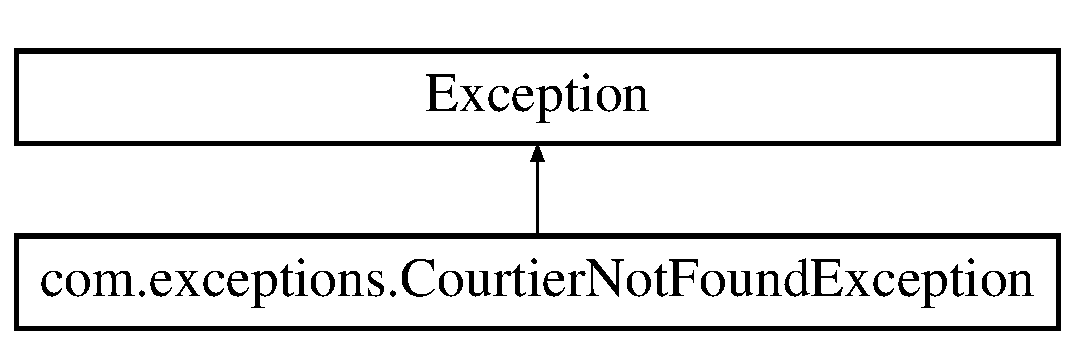
\includegraphics[height=2.000000cm]{classcom_1_1exceptions_1_1_courtier_not_found_exception}
\end{center}
\end{figure}
\subsection*{Public Member Functions}
\begin{DoxyCompactItemize}
\item 
\mbox{\Hypertarget{classcom_1_1exceptions_1_1_courtier_not_found_exception_a90866e2d3c1d03a63ef5e50238ef0252}\label{classcom_1_1exceptions_1_1_courtier_not_found_exception_a90866e2d3c1d03a63ef5e50238ef0252}} 
{\bfseries Courtier\+Not\+Found\+Exception} (String msg)
\item 
\mbox{\Hypertarget{classcom_1_1exceptions_1_1_courtier_not_found_exception_ada8c1148ac23a912559bc98d67295bca}\label{classcom_1_1exceptions_1_1_courtier_not_found_exception_ada8c1148ac23a912559bc98d67295bca}} 
String {\bfseries get\+Message} ()
\end{DoxyCompactItemize}


The documentation for this class was generated from the following file\+:\begin{DoxyCompactItemize}
\item 
C\+:/\+Users/\+Nick/\+Desktop/\+M1 M\+I\+A\+G\+E/\+Iam\+The\+One/\+Systèmes \& Algo Répartis/\+Projet/sar/src/com/exceptions/Courtier\+Not\+Found\+Exception.\+java\end{DoxyCompactItemize}

\hypertarget{classcom_1_1m1sar_1_1_entreprise}{}\section{com.\+m1sar.\+Entreprise Class Reference}
\label{classcom_1_1m1sar_1_1_entreprise}\index{com.\+m1sar.\+Entreprise@{com.\+m1sar.\+Entreprise}}
\subsection*{Public Member Functions}
\begin{DoxyCompactItemize}
\item 
\mbox{\Hypertarget{classcom_1_1m1sar_1_1_entreprise_a0d94dc249f273f6d1fe6222b362934c8}\label{classcom_1_1m1sar_1_1_entreprise_a0d94dc249f273f6d1fe6222b362934c8}} 
int {\bfseries get\+Nb\+Demandes\+Achats} ()
\item 
\mbox{\Hypertarget{classcom_1_1m1sar_1_1_entreprise_a091eac6f864b9c034c7ae7b6a96bb113}\label{classcom_1_1m1sar_1_1_entreprise_a091eac6f864b9c034c7ae7b6a96bb113}} 
void {\bfseries set\+Nb\+Demandes\+Achats} (int nb\+Demandes\+Achats)
\item 
\mbox{\Hypertarget{classcom_1_1m1sar_1_1_entreprise_a9378c606d234ccd1668e192fa6dc7dc9}\label{classcom_1_1m1sar_1_1_entreprise_a9378c606d234ccd1668e192fa6dc7dc9}} 
int {\bfseries get\+Nb\+Demande\+Ventes} ()
\item 
\mbox{\Hypertarget{classcom_1_1m1sar_1_1_entreprise_a4c63797f5fc51ab760890e5d0137681c}\label{classcom_1_1m1sar_1_1_entreprise_a4c63797f5fc51ab760890e5d0137681c}} 
void {\bfseries set\+Nb\+Demande\+Ventes} (int nb\+Demande\+Ventes)
\item 
\mbox{\Hypertarget{classcom_1_1m1sar_1_1_entreprise_a504a5cb6bb3e40abc4e13bd8c8957144}\label{classcom_1_1m1sar_1_1_entreprise_a504a5cb6bb3e40abc4e13bd8c8957144}} 
{\bfseries Entreprise} (String name, int nb\+Actions, double prix\+Unitaire\+Action)
\item 
\mbox{\Hypertarget{classcom_1_1m1sar_1_1_entreprise_a585df0a1e4be7b7b635b9d724b40d4af}\label{classcom_1_1m1sar_1_1_entreprise_a585df0a1e4be7b7b635b9d724b40d4af}} 
int {\bfseries get\+Nb\+Actions} ()
\item 
\mbox{\Hypertarget{classcom_1_1m1sar_1_1_entreprise_a53c34b65f323f707adfc60abeab0366a}\label{classcom_1_1m1sar_1_1_entreprise_a53c34b65f323f707adfc60abeab0366a}} 
double {\bfseries get\+Prix\+Unitaire\+Action} ()
\item 
\mbox{\Hypertarget{classcom_1_1m1sar_1_1_entreprise_a83d6442a56f8aea7d43dfef97d797c76}\label{classcom_1_1m1sar_1_1_entreprise_a83d6442a56f8aea7d43dfef97d797c76}} 
void {\bfseries set\+Nb\+Actions} (int n)
\item 
\mbox{\Hypertarget{classcom_1_1m1sar_1_1_entreprise_af66aed31cdbaff6cefd61c2ec5b9bfe0}\label{classcom_1_1m1sar_1_1_entreprise_af66aed31cdbaff6cefd61c2ec5b9bfe0}} 
String {\bfseries get\+Name} ()
\item 
\mbox{\Hypertarget{classcom_1_1m1sar_1_1_entreprise_a0ed4009a7c3fc1269173bab119b36b3f}\label{classcom_1_1m1sar_1_1_entreprise_a0ed4009a7c3fc1269173bab119b36b3f}} 
void {\bfseries set\+Prix\+Unitaire\+Action} (double n)
\item 
\mbox{\Hypertarget{classcom_1_1m1sar_1_1_entreprise_ae1ddae7b447940b42526dc9f4eaceb22}\label{classcom_1_1m1sar_1_1_entreprise_ae1ddae7b447940b42526dc9f4eaceb22}} 
String {\bfseries to\+String} ()
\item 
\mbox{\Hypertarget{classcom_1_1m1sar_1_1_entreprise_afdd74683ad48edc7c5c2ef7fc7cf93cc}\label{classcom_1_1m1sar_1_1_entreprise_afdd74683ad48edc7c5c2ef7fc7cf93cc}} 
void {\bfseries add\+Order} (\hyperlink{classcom_1_1m1sar_1_1_ordre}{Ordre} o)
\item 
\mbox{\Hypertarget{classcom_1_1m1sar_1_1_entreprise_a0696f7532e5b4b92e79625d9a180e4df}\label{classcom_1_1m1sar_1_1_entreprise_a0696f7532e5b4b92e79625d9a180e4df}} 
void {\bfseries Decrease\+Nb\+Actions} (int n)
\item 
\mbox{\Hypertarget{classcom_1_1m1sar_1_1_entreprise_a7263cbae806b5a15e9ada6319c52de13}\label{classcom_1_1m1sar_1_1_entreprise_a7263cbae806b5a15e9ada6319c52de13}} 
Vector$<$ \hyperlink{classcom_1_1m1sar_1_1_ordre}{Ordre} $>$ {\bfseries get\+Ordres} ()
\item 
\mbox{\Hypertarget{classcom_1_1m1sar_1_1_entreprise_af80280e108d6383f0ce6b788fc1b5316}\label{classcom_1_1m1sar_1_1_entreprise_af80280e108d6383f0ce6b788fc1b5316}} 
void {\bfseries decrease\+Nb\+Action} (int n)
\item 
\mbox{\Hypertarget{classcom_1_1m1sar_1_1_entreprise_a757cb487a04e7efa0c8af693e3fc0eb4}\label{classcom_1_1m1sar_1_1_entreprise_a757cb487a04e7efa0c8af693e3fc0eb4}} 
void {\bfseries inc\+Demandes\+Achat} ()
\item 
\mbox{\Hypertarget{classcom_1_1m1sar_1_1_entreprise_a83287630bd618f01257e26ecf714cca0}\label{classcom_1_1m1sar_1_1_entreprise_a83287630bd618f01257e26ecf714cca0}} 
void {\bfseries dec\+Demandes\+Achat} ()
\item 
\mbox{\Hypertarget{classcom_1_1m1sar_1_1_entreprise_a87ee28b2b1413b4fcb1cfeccc79a4d3a}\label{classcom_1_1m1sar_1_1_entreprise_a87ee28b2b1413b4fcb1cfeccc79a4d3a}} 
void {\bfseries inc\+Demandes\+Ventes} ()
\item 
\mbox{\Hypertarget{classcom_1_1m1sar_1_1_entreprise_a9c91ac39ef0a269a450731c94ed2108e}\label{classcom_1_1m1sar_1_1_entreprise_a9c91ac39ef0a269a450731c94ed2108e}} 
void {\bfseries dec\+Demandes\+Ventes} ()
\end{DoxyCompactItemize}


The documentation for this class was generated from the following file\+:\begin{DoxyCompactItemize}
\item 
C\+:/\+Users/\+Nick/\+Desktop/\+M1 M\+I\+A\+G\+E/\+Iam\+The\+One/\+Systèmes \& Algo Répartis/\+Projet/sar/src/com/m1sar/Entreprise.\+java\end{DoxyCompactItemize}

\hypertarget{classcom_1_1m1sar_1_1_fenetre}{}\section{com.\+m1sar.\+Fenetre Class Reference}
\label{classcom_1_1m1sar_1_1_fenetre}\index{com.\+m1sar.\+Fenetre@{com.\+m1sar.\+Fenetre}}
Inheritance diagram for com.\+m1sar.\+Fenetre\+:\begin{figure}[H]
\begin{center}
\leavevmode
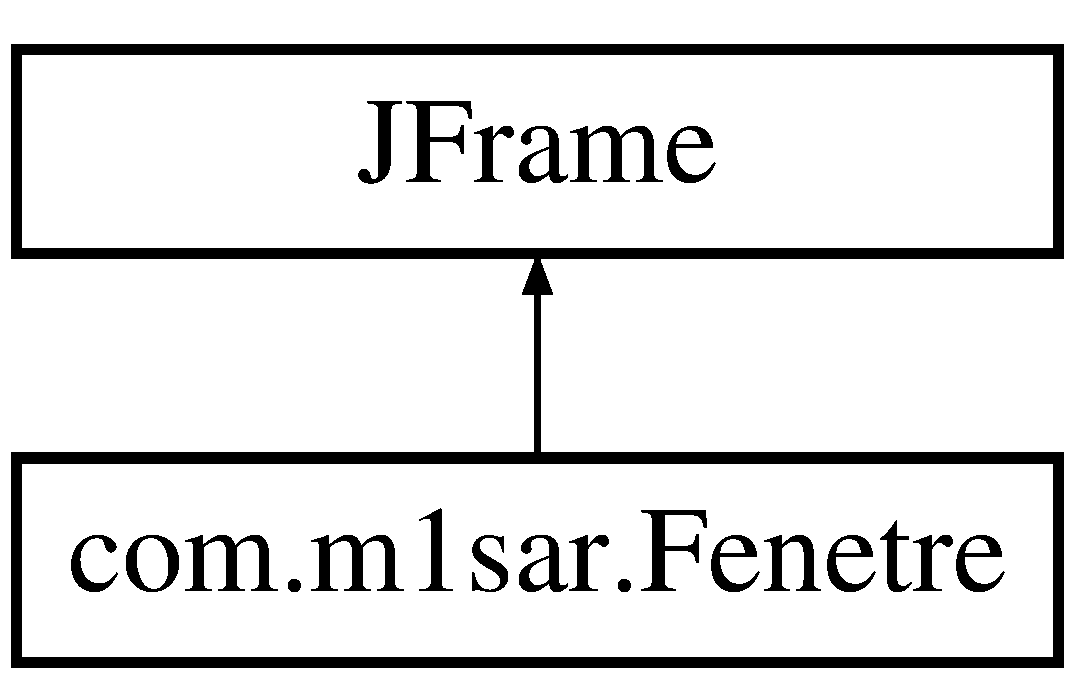
\includegraphics[height=2.000000cm]{classcom_1_1m1sar_1_1_fenetre}
\end{center}
\end{figure}
\subsection*{Classes}
\begin{DoxyCompactItemize}
\item 
class {\bfseries Bouton\+Listener}
\end{DoxyCompactItemize}
\subsection*{Public Member Functions}
\begin{DoxyCompactItemize}
\item 
\mbox{\Hypertarget{classcom_1_1m1sar_1_1_fenetre_ae780b07fb90122c68bcf59db05c1b615}\label{classcom_1_1m1sar_1_1_fenetre_ae780b07fb90122c68bcf59db05c1b615}} 
int {\bfseries get\+Portnb} ()
\item 
\mbox{\Hypertarget{classcom_1_1m1sar_1_1_fenetre_a8503e7f3d964cdd44447127e5129325b}\label{classcom_1_1m1sar_1_1_fenetre_a8503e7f3d964cdd44447127e5129325b}} 
void {\bfseries set\+Portnb} (int portnb)
\end{DoxyCompactItemize}


The documentation for this class was generated from the following file\+:\begin{DoxyCompactItemize}
\item 
C\+:/\+Users/\+Nick/\+Desktop/\+M1 M\+I\+A\+G\+E/\+Iam\+The\+One/\+Systèmes \& Algo Répartis/\+Projet/sar/src/com/m1sar/Fenetre.\+java\end{DoxyCompactItemize}

\hypertarget{classcom_1_1m1sar_1_1_ordre}{}\section{com.\+m1sar.\+Ordre Class Reference}
\label{classcom_1_1m1sar_1_1_ordre}\index{com.\+m1sar.\+Ordre@{com.\+m1sar.\+Ordre}}
Inheritance diagram for com.\+m1sar.\+Ordre\+:\begin{figure}[H]
\begin{center}
\leavevmode
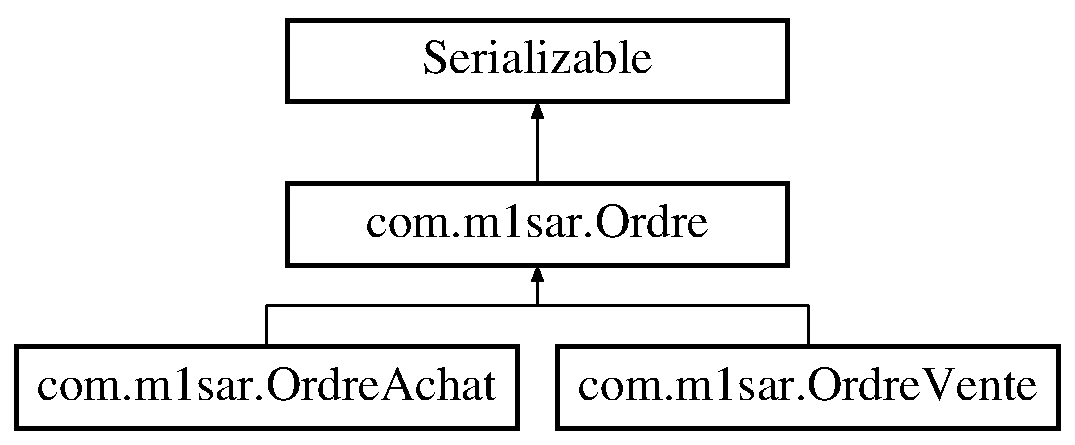
\includegraphics[height=3.000000cm]{classcom_1_1m1sar_1_1_ordre}
\end{center}
\end{figure}
\subsection*{Public Member Functions}
\begin{DoxyCompactItemize}
\item 
\mbox{\Hypertarget{classcom_1_1m1sar_1_1_ordre_a40d50192a295fa377b1955067e3b8455}\label{classcom_1_1m1sar_1_1_ordre_a40d50192a295fa377b1955067e3b8455}} 
boolean {\bfseries is\+Est\+Accepte} ()
\item 
\mbox{\Hypertarget{classcom_1_1m1sar_1_1_ordre_a42b1cc0fb374898ee7feb5335db1541d}\label{classcom_1_1m1sar_1_1_ordre_a42b1cc0fb374898ee7feb5335db1541d}} 
void {\bfseries set\+Est\+Accepte} (boolean \hyperlink{classcom_1_1m1sar_1_1_ordre_a7022809430ff96ce182601f7885d853c}{est\+Accepte})
\item 
\mbox{\Hypertarget{classcom_1_1m1sar_1_1_ordre_ac73cb37536a9b72f8b0dcb2504e5da2b}\label{classcom_1_1m1sar_1_1_ordre_ac73cb37536a9b72f8b0dcb2504e5da2b}} 
String {\bfseries get\+Nom\+Courtier} ()
\item 
\mbox{\Hypertarget{classcom_1_1m1sar_1_1_ordre_a67efcf96141aa33f891303e56a4e1996}\label{classcom_1_1m1sar_1_1_ordre_a67efcf96141aa33f891303e56a4e1996}} 
void {\bfseries set\+Nom\+Courtier} (String nom\+Courtier)
\item 
\mbox{\Hypertarget{classcom_1_1m1sar_1_1_ordre_a891dc1109048dd71c732b942d6fb82ea}\label{classcom_1_1m1sar_1_1_ordre_a891dc1109048dd71c732b942d6fb82ea}} 
{\bfseries Ordre} (String entreprise, String client, double prix\+\_\+\+Propose\+\_\+par\+\_\+\+Client, int quantite, String nom)
\item 
\mbox{\Hypertarget{classcom_1_1m1sar_1_1_ordre_a9528377ac85a5743487fc5cd799a2dce}\label{classcom_1_1m1sar_1_1_ordre_a9528377ac85a5743487fc5cd799a2dce}} 
String {\bfseries get\+Entreprise\+Name} ()
\item 
\mbox{\Hypertarget{classcom_1_1m1sar_1_1_ordre_ad7f04c3a54d48f2d49f5b9a92861072d}\label{classcom_1_1m1sar_1_1_ordre_ad7f04c3a54d48f2d49f5b9a92861072d}} 
double {\bfseries get\+Prix\+Unitaire} ()
\item 
void \hyperlink{classcom_1_1m1sar_1_1_ordre_aabc1a386ae20e7aa15391de8c2ab0062}{set\+Est\+Fini} ()
\item 
\mbox{\Hypertarget{classcom_1_1m1sar_1_1_ordre_aaa2f967373a08a112418e8056fd31f2e}\label{classcom_1_1m1sar_1_1_ordre_aaa2f967373a08a112418e8056fd31f2e}} 
int {\bfseries get\+Id} ()
\item 
\mbox{\Hypertarget{classcom_1_1m1sar_1_1_ordre_ab6c7bc3c700bd50cb0e27f101b3faae2}\label{classcom_1_1m1sar_1_1_ordre_ab6c7bc3c700bd50cb0e27f101b3faae2}} 
void {\bfseries set\+Id} (int id)
\item 
\mbox{\Hypertarget{classcom_1_1m1sar_1_1_ordre_a206ed238c2faba3586f21832cbf28d59}\label{classcom_1_1m1sar_1_1_ordre_a206ed238c2faba3586f21832cbf28d59}} 
String {\bfseries to\+String} ()
\item 
\mbox{\Hypertarget{classcom_1_1m1sar_1_1_ordre_a89c5590f532e59c0af9e23c834c0aa8e}\label{classcom_1_1m1sar_1_1_ordre_a89c5590f532e59c0af9e23c834c0aa8e}} 
int {\bfseries get\+Quantite\+Client} ()
\item 
\mbox{\Hypertarget{classcom_1_1m1sar_1_1_ordre_a56112d1939a3bbdf6c789349083342f9}\label{classcom_1_1m1sar_1_1_ordre_a56112d1939a3bbdf6c789349083342f9}} 
void {\bfseries set\+Quantite\+Client} (int quantite\+Client)
\end{DoxyCompactItemize}
\subsection*{Public Attributes}
\begin{DoxyCompactItemize}
\item 
boolean \hyperlink{classcom_1_1m1sar_1_1_ordre_a7022809430ff96ce182601f7885d853c}{est\+Accepte} =false
\end{DoxyCompactItemize}


\subsection{Member Function Documentation}
\mbox{\Hypertarget{classcom_1_1m1sar_1_1_ordre_aabc1a386ae20e7aa15391de8c2ab0062}\label{classcom_1_1m1sar_1_1_ordre_aabc1a386ae20e7aa15391de8c2ab0062}} 
\index{com\+::m1sar\+::\+Ordre@{com\+::m1sar\+::\+Ordre}!set\+Est\+Fini@{set\+Est\+Fini}}
\index{set\+Est\+Fini@{set\+Est\+Fini}!com\+::m1sar\+::\+Ordre@{com\+::m1sar\+::\+Ordre}}
\subsubsection{\texorpdfstring{set\+Est\+Fini()}{setEstFini()}}
{\footnotesize\ttfamily void com.\+m1sar.\+Ordre.\+set\+Est\+Fini (\begin{DoxyParamCaption}{ }\end{DoxyParamCaption})}

\begin{DoxyAuthor}{Author}
Lyes Sets the order as an accomplished order 
\end{DoxyAuthor}


\subsection{Member Data Documentation}
\mbox{\Hypertarget{classcom_1_1m1sar_1_1_ordre_a7022809430ff96ce182601f7885d853c}\label{classcom_1_1m1sar_1_1_ordre_a7022809430ff96ce182601f7885d853c}} 
\index{com\+::m1sar\+::\+Ordre@{com\+::m1sar\+::\+Ordre}!est\+Accepte@{est\+Accepte}}
\index{est\+Accepte@{est\+Accepte}!com\+::m1sar\+::\+Ordre@{com\+::m1sar\+::\+Ordre}}
\subsubsection{\texorpdfstring{est\+Accepte}{estAccepte}}
{\footnotesize\ttfamily boolean com.\+m1sar.\+Ordre.\+est\+Accepte =false}

Tells if the order is finished 

The documentation for this class was generated from the following file\+:\begin{DoxyCompactItemize}
\item 
C\+:/\+Users/\+Nick/\+Desktop/\+M1 M\+I\+A\+G\+E/\+Iam\+The\+One/\+Systèmes \& Algo Répartis/\+Projet/sar/src/com/m1sar/Ordre.\+java\end{DoxyCompactItemize}

\hypertarget{classcom_1_1m1sar_1_1_ordre_achat}{}\section{com.\+m1sar.\+Ordre\+Achat Class Reference}
\label{classcom_1_1m1sar_1_1_ordre_achat}\index{com.\+m1sar.\+Ordre\+Achat@{com.\+m1sar.\+Ordre\+Achat}}
Inheritance diagram for com.\+m1sar.\+Ordre\+Achat\+:\begin{figure}[H]
\begin{center}
\leavevmode
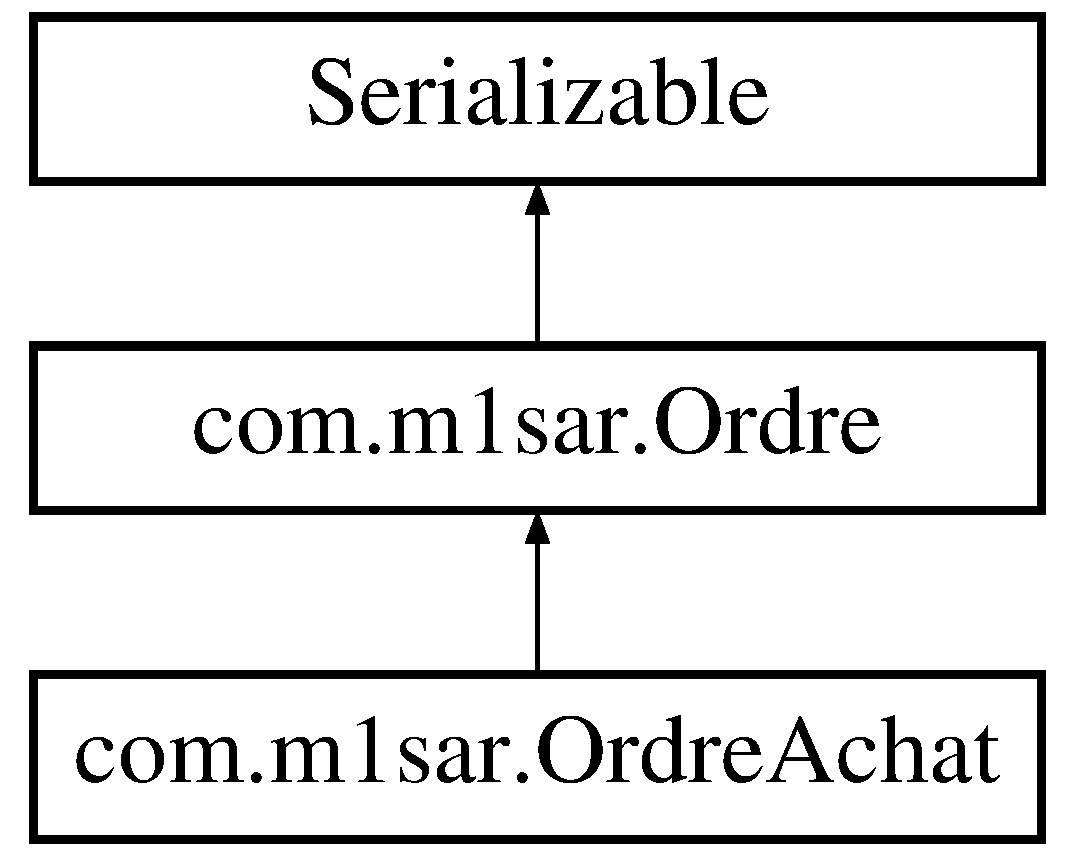
\includegraphics[height=3.000000cm]{classcom_1_1m1sar_1_1_ordre_achat}
\end{center}
\end{figure}
\subsection*{Public Member Functions}
\begin{DoxyCompactItemize}
\item 
\mbox{\Hypertarget{classcom_1_1m1sar_1_1_ordre_achat_a5448a8f8859556109bbbbcbf136f40cb}\label{classcom_1_1m1sar_1_1_ordre_achat_a5448a8f8859556109bbbbcbf136f40cb}} 
{\bfseries Ordre\+Achat} (String entreprise, String client, double prix\+\_\+\+Propose\+\_\+par\+\_\+\+Client, int quantite, String nom)
\end{DoxyCompactItemize}
\subsection*{Additional Inherited Members}


The documentation for this class was generated from the following file\+:\begin{DoxyCompactItemize}
\item 
C\+:/\+Users/\+Nick/\+Desktop/\+M1 M\+I\+A\+G\+E/\+Iam\+The\+One/\+Systèmes \& Algo Répartis/\+Projet/sar/src/com/m1sar/Ordre\+Achat.\+java\end{DoxyCompactItemize}

\hypertarget{classcom_1_1m1sar_1_1_ordre_vente}{}\section{com.\+m1sar.\+Ordre\+Vente Class Reference}
\label{classcom_1_1m1sar_1_1_ordre_vente}\index{com.\+m1sar.\+Ordre\+Vente@{com.\+m1sar.\+Ordre\+Vente}}
Inheritance diagram for com.\+m1sar.\+Ordre\+Vente\+:\begin{figure}[H]
\begin{center}
\leavevmode
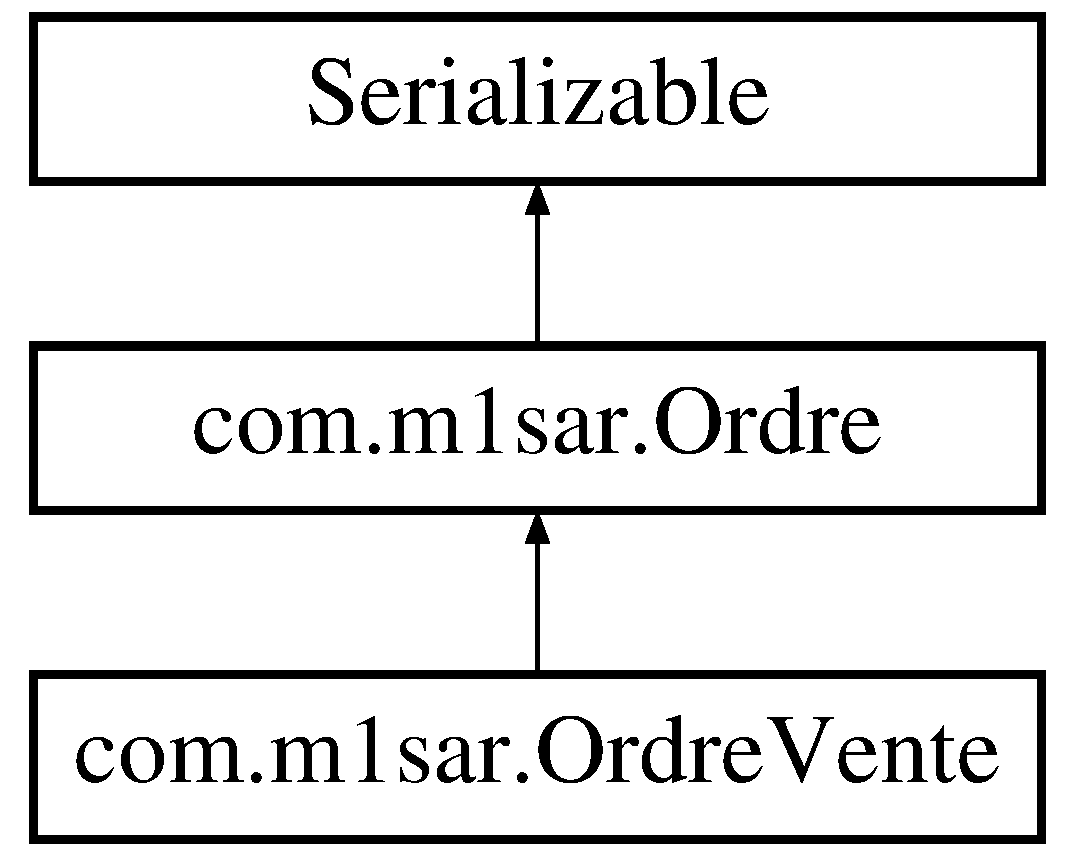
\includegraphics[height=3.000000cm]{classcom_1_1m1sar_1_1_ordre_vente}
\end{center}
\end{figure}
\subsection*{Public Member Functions}
\begin{DoxyCompactItemize}
\item 
\mbox{\Hypertarget{classcom_1_1m1sar_1_1_ordre_vente_ac6f7721569e4d4bbc186a3dbf4b5bd5b}\label{classcom_1_1m1sar_1_1_ordre_vente_ac6f7721569e4d4bbc186a3dbf4b5bd5b}} 
{\bfseries Ordre\+Vente} (String entreprise, String client, double prix\+\_\+\+Propose\+\_\+par\+\_\+\+Client, int quantite, String nom)
\end{DoxyCompactItemize}
\subsection*{Additional Inherited Members}


The documentation for this class was generated from the following file\+:\begin{DoxyCompactItemize}
\item 
C\+:/\+Users/\+Nick/\+Desktop/\+M1 M\+I\+A\+G\+E/\+Iam\+The\+One/\+Systèmes \& Algo Répartis/\+Projet/sar/src/com/m1sar/Ordre\+Vente.\+java\end{DoxyCompactItemize}

\hypertarget{classcom_1_1m1sar_1_1_thread_bourse}{}\section{com.\+m1sar.\+Thread\+Bourse Class Reference}
\label{classcom_1_1m1sar_1_1_thread_bourse}\index{com.\+m1sar.\+Thread\+Bourse@{com.\+m1sar.\+Thread\+Bourse}}
Inheritance diagram for com.\+m1sar.\+Thread\+Bourse\+:\begin{figure}[H]
\begin{center}
\leavevmode
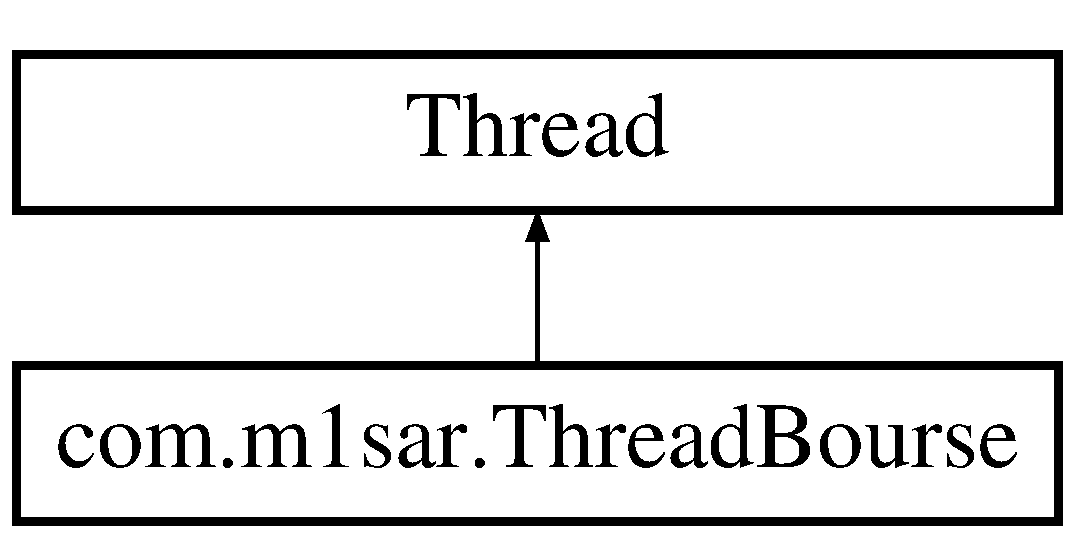
\includegraphics[height=2.000000cm]{classcom_1_1m1sar_1_1_thread_bourse}
\end{center}
\end{figure}
\subsection*{Public Member Functions}
\begin{DoxyCompactItemize}
\item 
\mbox{\Hypertarget{classcom_1_1m1sar_1_1_thread_bourse_ac083c16dd85a59f19f3ea1728d32e057}\label{classcom_1_1m1sar_1_1_thread_bourse_ac083c16dd85a59f19f3ea1728d32e057}} 
{\bfseries Thread\+Bourse} (Socket s\+Courtier, int nport, \hyperlink{classcom_1_1m1sar_1_1_bourse}{Bourse} b, String nom)
\item 
\mbox{\Hypertarget{classcom_1_1m1sar_1_1_thread_bourse_ac052e73112ac20e1c2e6fa3f7c9bce94}\label{classcom_1_1m1sar_1_1_thread_bourse_ac052e73112ac20e1c2e6fa3f7c9bce94}} 
void {\bfseries connexion\+Courtier} ()
\item 
\mbox{\Hypertarget{classcom_1_1m1sar_1_1_thread_bourse_adfc535a296af8c294920dadf497a928b}\label{classcom_1_1m1sar_1_1_thread_bourse_adfc535a296af8c294920dadf497a928b}} 
String {\bfseries get\+Nom\+Courtier} ()
\item 
\mbox{\Hypertarget{classcom_1_1m1sar_1_1_thread_bourse_aa7c0c87d2fb28b192bf812ae0654d596}\label{classcom_1_1m1sar_1_1_thread_bourse_aa7c0c87d2fb28b192bf812ae0654d596}} 
void {\bfseries set\+Nom\+Courtier} (String nom\+Courtier)
\item 
\mbox{\Hypertarget{classcom_1_1m1sar_1_1_thread_bourse_a5d851ffad404a8c62a3175f222ce410f}\label{classcom_1_1m1sar_1_1_thread_bourse_a5d851ffad404a8c62a3175f222ce410f}} 
void {\bfseries run} ()
\item 
void \hyperlink{classcom_1_1m1sar_1_1_thread_bourse_acea1b4e4e2757b3cc82bba756eda4057}{send\+Price\+Companies} ()  throws I\+O\+Exception 
\item 
void \hyperlink{classcom_1_1m1sar_1_1_thread_bourse_a714db4602cd1dff9a732caf861b1d5e6}{Sur\+Reception\+De} (\hyperlink{classcom_1_1m1sar_1_1_ordre}{Ordre} ordre)
\item 
void \hyperlink{classcom_1_1m1sar_1_1_thread_bourse_a431e283fa57268481834f67709b7ec07}{envoyer\+Rep} (int id, boolean rep)  throws I\+O\+Exception 
\item 
\mbox{\Hypertarget{classcom_1_1m1sar_1_1_thread_bourse_a7fe473194bcccaa0aa31b8f0e816834b}\label{classcom_1_1m1sar_1_1_thread_bourse_a7fe473194bcccaa0aa31b8f0e816834b}} 
void {\bfseries inc\+Nb\+Client} ()
\item 
\mbox{\Hypertarget{classcom_1_1m1sar_1_1_thread_bourse_a2b4318d2553102b0421c5616a7ef93e9}\label{classcom_1_1m1sar_1_1_thread_bourse_a2b4318d2553102b0421c5616a7ef93e9}} 
boolean {\bfseries est\+Dispo} ()
\item 
\mbox{\Hypertarget{classcom_1_1m1sar_1_1_thread_bourse_aa9a44f7d1cd2d2cfce8520270b2cd7f8}\label{classcom_1_1m1sar_1_1_thread_bourse_aa9a44f7d1cd2d2cfce8520270b2cd7f8}} 
int {\bfseries get\+Nport} ()
\item 
\mbox{\Hypertarget{classcom_1_1m1sar_1_1_thread_bourse_a54c11ec3c4ecf3235a66e457ba464c39}\label{classcom_1_1m1sar_1_1_thread_bourse_a54c11ec3c4ecf3235a66e457ba464c39}} 
Inet\+Address {\bfseries get\+Inet\+Address} ()
\end{DoxyCompactItemize}


\subsection{Member Function Documentation}
\mbox{\Hypertarget{classcom_1_1m1sar_1_1_thread_bourse_a431e283fa57268481834f67709b7ec07}\label{classcom_1_1m1sar_1_1_thread_bourse_a431e283fa57268481834f67709b7ec07}} 
\index{com\+::m1sar\+::\+Thread\+Bourse@{com\+::m1sar\+::\+Thread\+Bourse}!envoyer\+Rep@{envoyer\+Rep}}
\index{envoyer\+Rep@{envoyer\+Rep}!com\+::m1sar\+::\+Thread\+Bourse@{com\+::m1sar\+::\+Thread\+Bourse}}
\subsubsection{\texorpdfstring{envoyer\+Rep()}{envoyerRep()}}
{\footnotesize\ttfamily void com.\+m1sar.\+Thread\+Bourse.\+envoyer\+Rep (\begin{DoxyParamCaption}\item[{int}]{id,  }\item[{boolean}]{rep }\end{DoxyParamCaption}) throws I\+O\+Exception}

Answers to the broker if the order is ok or not 
\begin{DoxyParams}{Parameters}
{\em id} & \+: the id of the broker  \+: the answere \+: true/false \\
\hline
\end{DoxyParams}
\mbox{\Hypertarget{classcom_1_1m1sar_1_1_thread_bourse_acea1b4e4e2757b3cc82bba756eda4057}\label{classcom_1_1m1sar_1_1_thread_bourse_acea1b4e4e2757b3cc82bba756eda4057}} 
\index{com\+::m1sar\+::\+Thread\+Bourse@{com\+::m1sar\+::\+Thread\+Bourse}!send\+Price\+Companies@{send\+Price\+Companies}}
\index{send\+Price\+Companies@{send\+Price\+Companies}!com\+::m1sar\+::\+Thread\+Bourse@{com\+::m1sar\+::\+Thread\+Bourse}}
\subsubsection{\texorpdfstring{send\+Price\+Companies()}{sendPriceCompanies()}}
{\footnotesize\ttfamily void com.\+m1sar.\+Thread\+Bourse.\+send\+Price\+Companies (\begin{DoxyParamCaption}{ }\end{DoxyParamCaption}) throws I\+O\+Exception}

the brocker sends to his customers the information about the share parices of each company in the stock market \mbox{\Hypertarget{classcom_1_1m1sar_1_1_thread_bourse_a714db4602cd1dff9a732caf861b1d5e6}\label{classcom_1_1m1sar_1_1_thread_bourse_a714db4602cd1dff9a732caf861b1d5e6}} 
\index{com\+::m1sar\+::\+Thread\+Bourse@{com\+::m1sar\+::\+Thread\+Bourse}!Sur\+Reception\+De@{Sur\+Reception\+De}}
\index{Sur\+Reception\+De@{Sur\+Reception\+De}!com\+::m1sar\+::\+Thread\+Bourse@{com\+::m1sar\+::\+Thread\+Bourse}}
\subsubsection{\texorpdfstring{Sur\+Reception\+De()}{SurReceptionDe()}}
{\footnotesize\ttfamily void com.\+m1sar.\+Thread\+Bourse.\+Sur\+Reception\+De (\begin{DoxyParamCaption}\item[{\hyperlink{classcom_1_1m1sar_1_1_ordre}{Ordre}}]{ordre }\end{DoxyParamCaption})}


\begin{DoxyParams}{Parameters}
{\em ordre} & the order passed by the customer send the order to the stock market \\
\hline
\end{DoxyParams}


The documentation for this class was generated from the following file\+:\begin{DoxyCompactItemize}
\item 
C\+:/\+Users/\+Nick/\+Desktop/\+M1 M\+I\+A\+G\+E/\+Iam\+The\+One/\+Systèmes \& Algo Répartis/\+Projet/sar/src/com/m1sar/Thread\+Bourse.\+java\end{DoxyCompactItemize}

%--- End generated contents ---

% Index
\backmatter
\newpage
\phantomsection
\clearemptydoublepage
\addcontentsline{toc}{chapter}{Index}
\printindex

\end{document}
